\chapter{Concluzii și rezultate}

\section{Rezultate experimentale}

Pentru evaluarea modelului AI, au fost realizate mai multe experimente controlate asupra problemei de reconstrucție binară a matricei unui cod QR. Scopul acestor experimente a fost verificarea capacității modelului de a transforma o imagine QR, de dimensiune $210 \times 210$, într-o matrice binară de dimensiune $21 \times 21$, unde fiecare element reprezintă un modul al codului QR.

Setul de date utilizat conține $10000$ de imagini, iar împărțirea a fost realizată în două subseturi: $8000$ imagini pentru antrenare și $2000$ imagini pentru validare. Nu a mai fost folosit un set de test separat, deoarece scopul principal al experimentelor a fost compararea controlată a configurațiilor pe același set de validare. Împărțirea a fost realizată folosind un seed fix, egal cu $42$, pentru ca rezultatele să poată fi reproduse.

Deoarece fiecare cod QR are $21 \times 21 = 441$ module, setul de validare conține în total:

\[
    2000 \times 441 = 882000
\]

predicții binare la nivel de modul QR.

Pentru evaluare s-au folosit mai multe metrici, însă comparația principală dintre experimente a fost realizată pe baza ratei erorii la nivel de bit pe setul de validare. Această metrică măsoară proporția modulelor QR prezise greșit. În mod echivalent, acuratețea la nivel de bit este complementul acesteia.

\[
    BER = \frac{FP + FN}{TP + TN + FP + FN}
\]

\[
    BitAccuracy = 1 - BER
\]

A fost urmărită și acuratețea exactă la nivel de cod QR, care consideră o imagine corectă doar dacă toate cele $441$ de module ale sale au fost prezise corect. Această metrică este mult mai strictă, deoarece o singură eroare de bit face ca întreaga reconstrucție QR să fie considerată greșită.

\[
    ExactAccuracy = \frac{N_{QR\ corecte}}{N_{QR\ total}}
\]

În cadrul experimentelor au fost rulate $11$ configurații, fiecare timp de $30$ de epoci. Nu a fost realizată o căutare full factorial, ci o serie de experimente controlate, grupate în patru categorii. Modelul de bază a folosit arhitectura cu batch size $32$, rata de învățare $10^{-4}$, weight decay $10^{-4}$ și dropout fix $0.04$.

Experimentele au fost următoarele: 2 experimente pentru batch size, 3 experimente pentru learning rate, 3 experimente pentru weight decay, 3 experimente pentru comparația arhitecturilor. Astfel, numărul total de experimente a fost 11.

Valorile testate pentru batch size au fost:

\[
    batchSize \in \{16, 32\}
\]

Valorile testate pentru rata de învățare au fost:

\[
    lr \in \{5 \cdot 10^{-4}, 10^{-4}, 5 \cdot 10^{-5}\}
\]

Valorile testate pentru regularizare au fost:

\[
    weightDecay \in \{0, 10^{-4}, 10^{-3}\}
\]

Pentru arhitectură au fost comparate trei variante: \textit{arch\_small}, \textit{arch\_baseline} și \textit{arch\_large}. Varianta \textit{arch\_small} a folosit $546001$ parametri, varianta \textit{arch\_baseline} a folosit $2769313$ parametri, iar varianta \textit{arch\_large} a folosit $3360161$ parametri.

\begin{figure}[htbp]
    \centering
    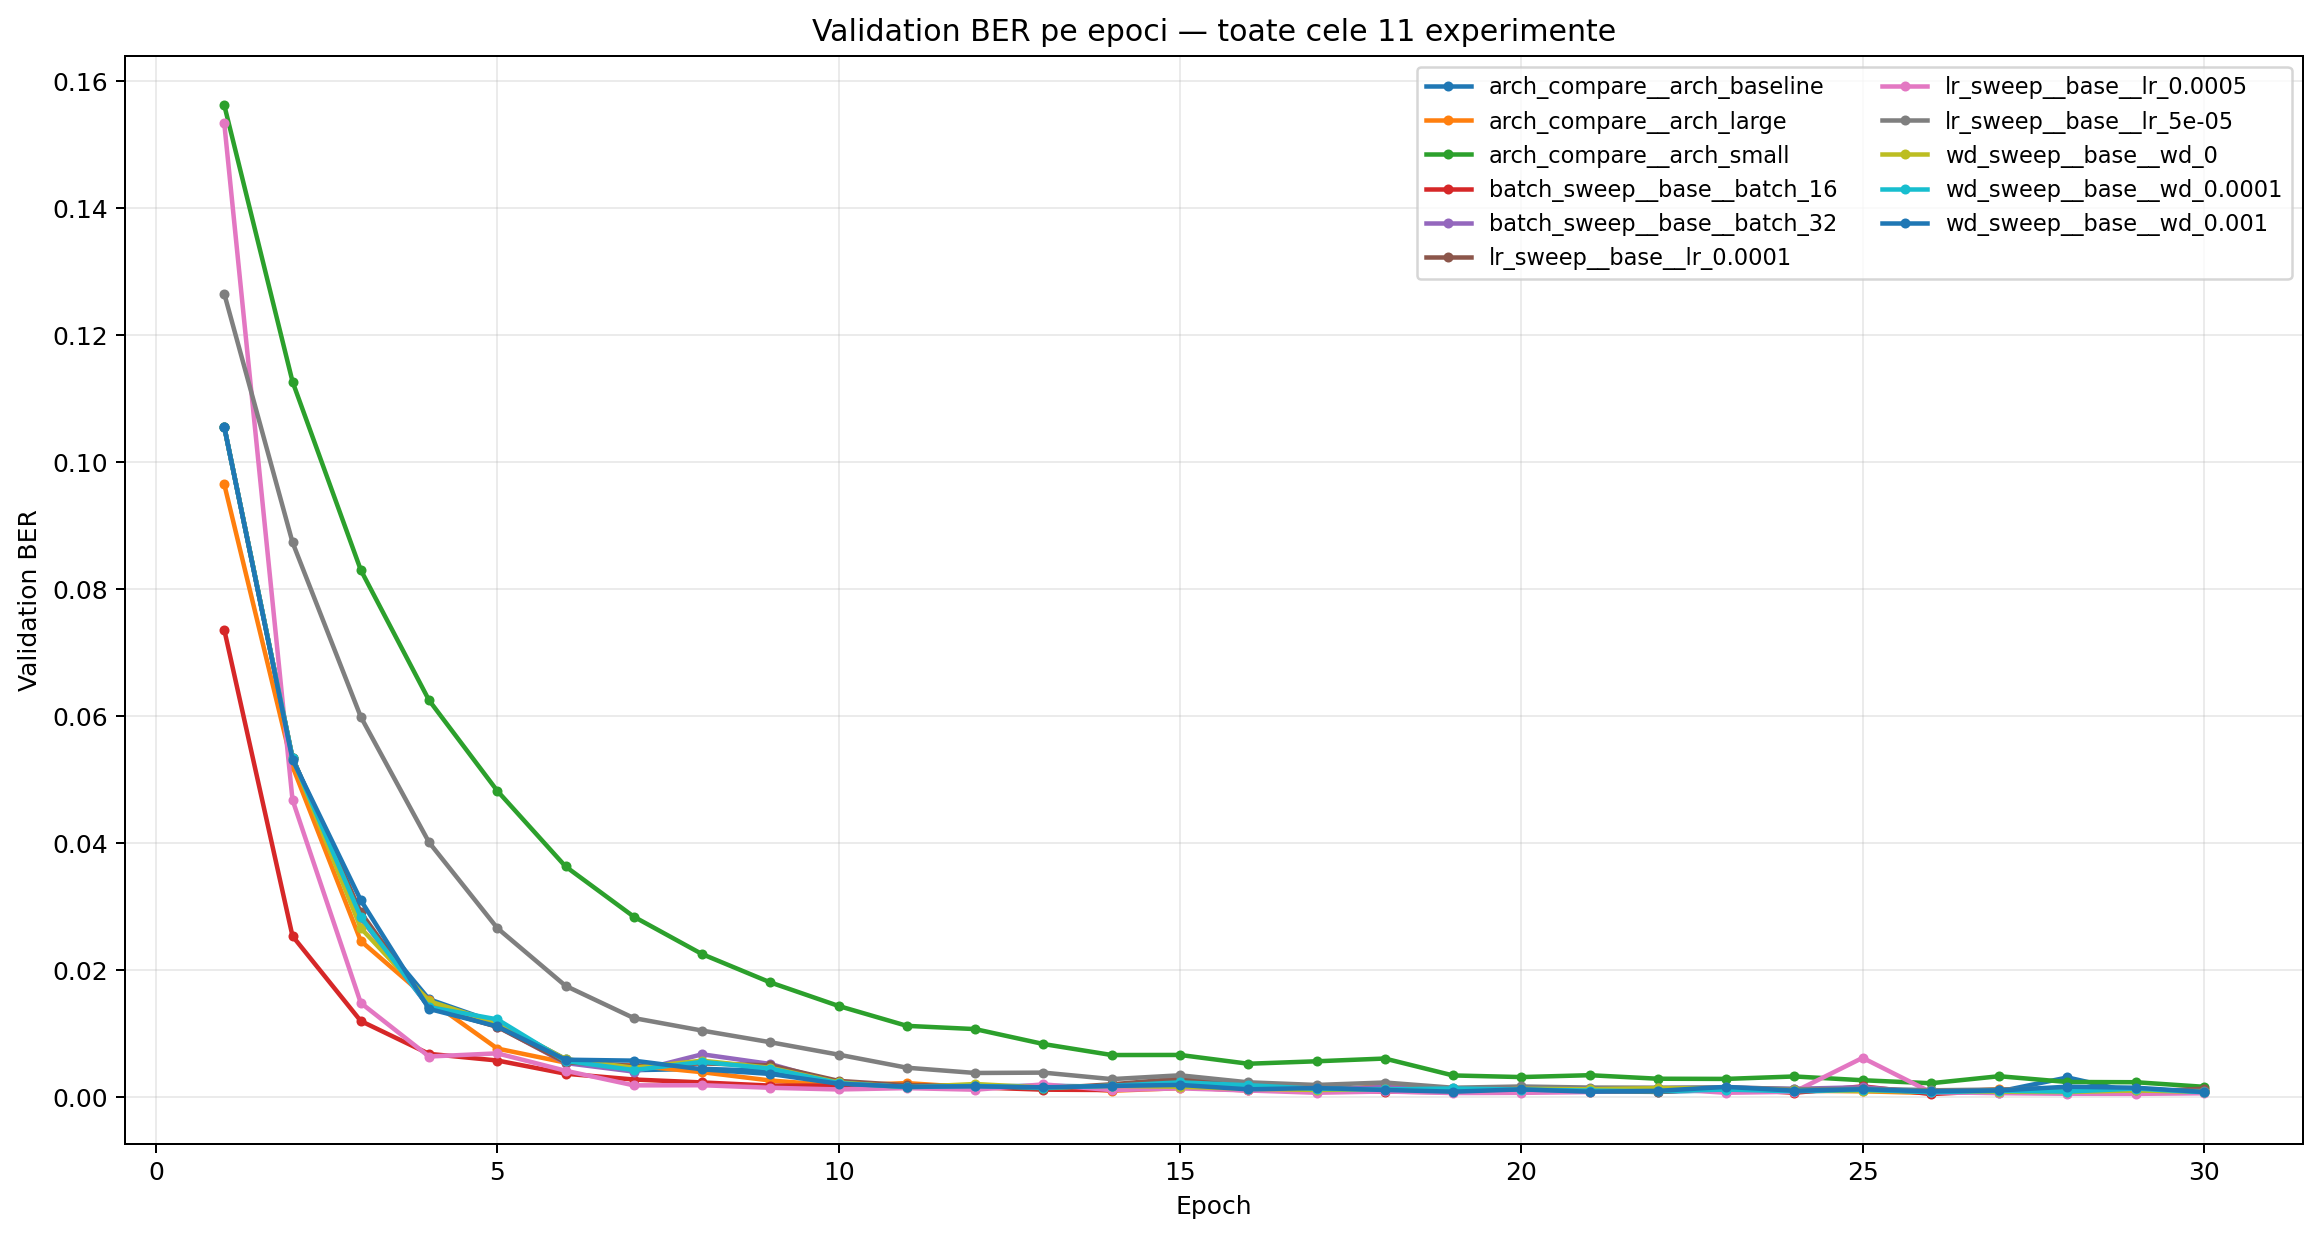
\includegraphics[width=0.8\textwidth]{images/01_all_experiments_val_ber_by_epoch.png}
    \caption{Evoluția ratei erorii la nivel de bit pe setul de validare pentru toate cele 11 experimente}
\end{figure}
\FloatBarrier

\begin{figure}[htbp]
    \centering
    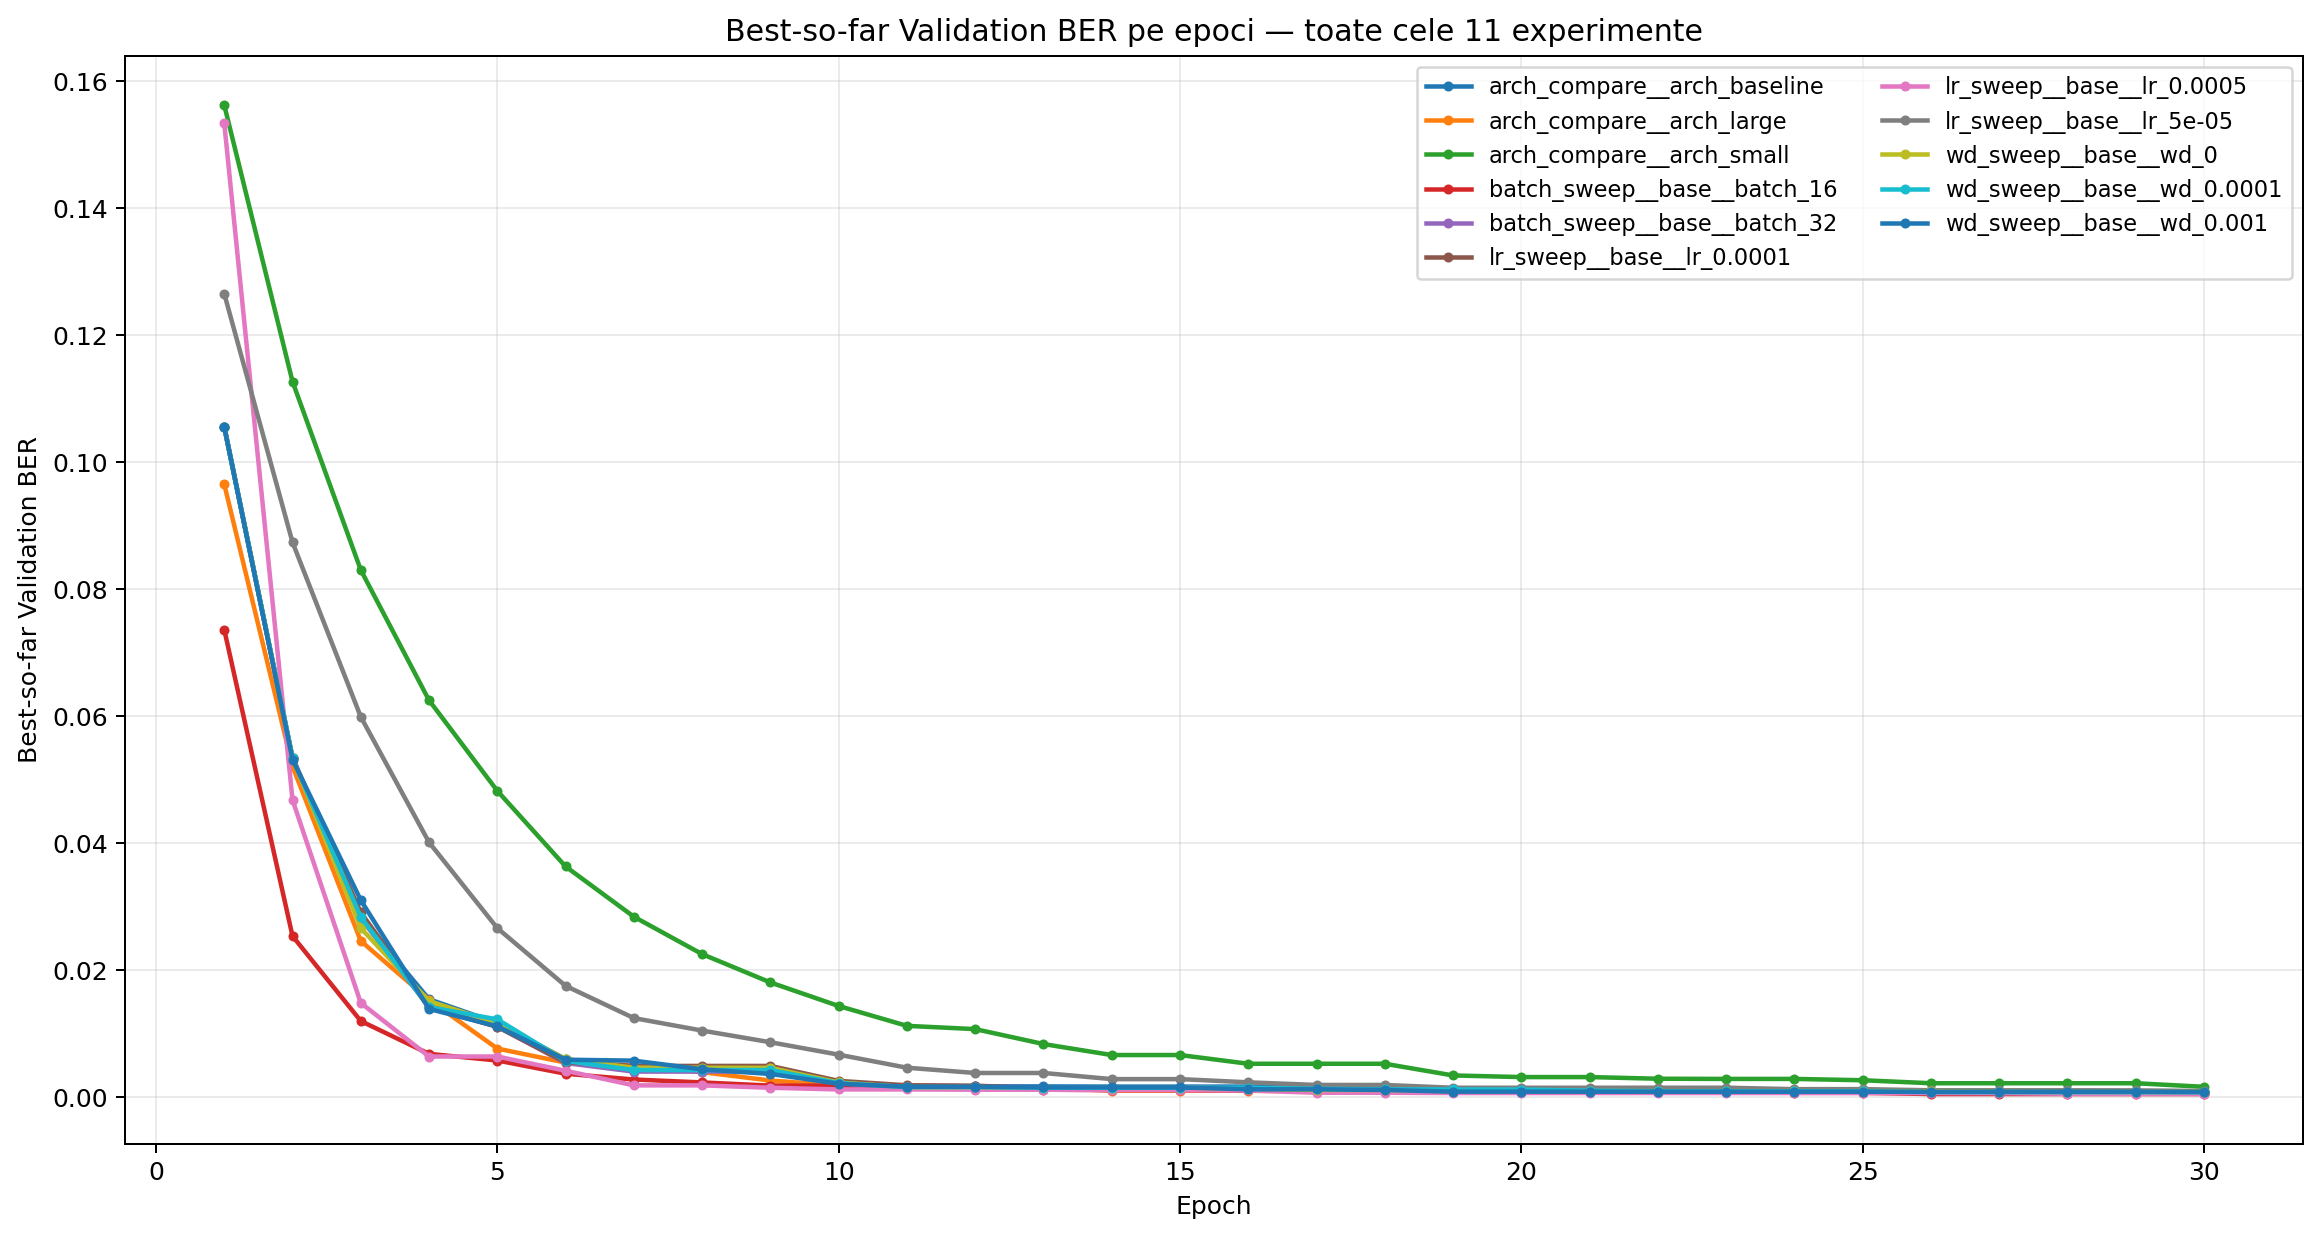
\includegraphics[width=0.8\textwidth]{images/02_all_experiments_best_so_far_val_ber_by_epoch.png}
    \caption{Evoluția celui mai bun BER obținut până la fiecare epocă pentru toate experimentele}
\end{figure}
\FloatBarrier

\begin{figure}[htbp]
    \centering
    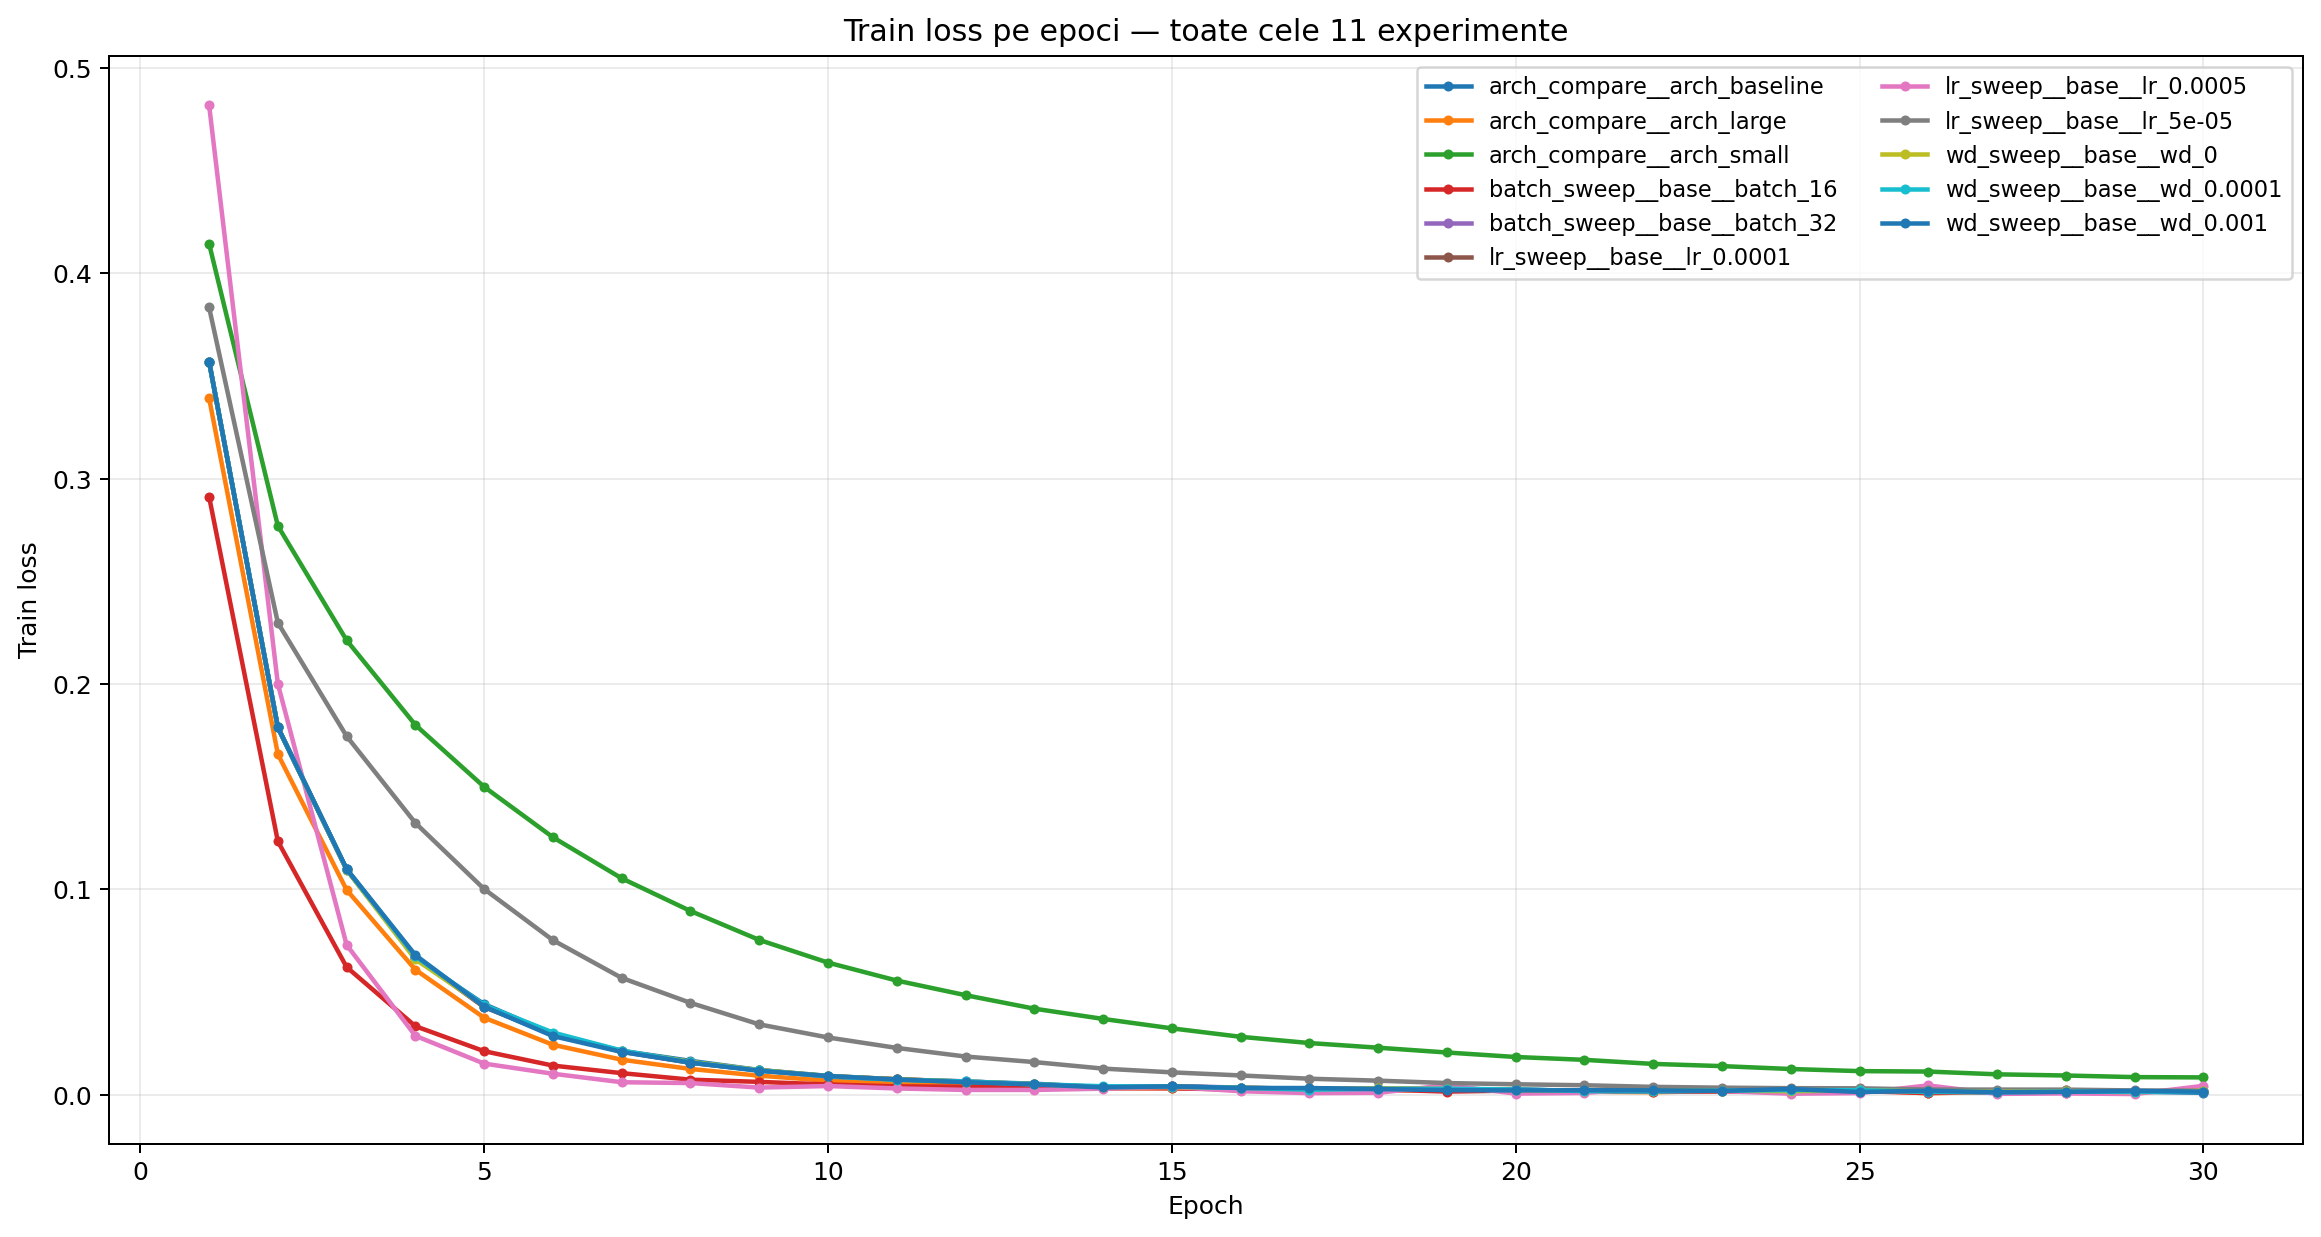
\includegraphics[width=0.8\textwidth]{images/03_all_experiments_train_loss_by_epoch.png}
    \caption{Evoluția funcției de pierdere pe setul de antrenare pentru toate experimentele}
\end{figure}
\FloatBarrier

Rezultatele principale obținute pentru cele $11$ experimente sunt prezentate în tabelul următor. Configurațiile sunt ordonate după cea mai mică valoare a metricii $val\_ber$ obținută în timpul celor $30$ de epoci.

\begin{table}[htbp]
    \centering
    \small
    \resizebox{\textwidth}{!}{
    \begin{tabular}{|l|l|c|c|c|c|c|c|}
        \hline
        \textbf{Experiment} & \textbf{Variantă} & \textbf{Epocă} & \textbf{Best BER} & \textbf{Final BER} & \textbf{Erori/QR} & \textbf{Timp total} & \textbf{Parametri} \\
        \hline
        batch\_sweep\_\_base\_\_batch\_16 & batch=$16$ & 26 & 0.0455\% & 0.0757\% & 0.2005 & 92.75 min & 2769313 \\
        \hline
        lr\_sweep\_\_base\_\_lr\_0.0005 & lr=$5 \cdot 10^{-4}$ & 29 & 0.0485\% & 0.0580\% & 0.2140 & 108.25 min & 2769313 \\
        \hline
        arch\_compare\_\_arch\_large & arch\_large & 26 & 0.0618\% & 0.0766\% & 0.2725 & 127.50 min & 3360161 \\
        \hline
        arch\_compare\_\_arch\_baseline & arch\_baseline & 29 & 0.0654\% & 0.0872\% & 0.2885 & 141.84 min & 2769313 \\
        \hline
        batch\_sweep\_\_base\_\_batch\_32 & batch=$32$ & 28 & 0.0678\% & 0.0770\% & 0.2990 & 117.49 min & 2769313 \\
        \hline
        lr\_sweep\_\_base\_\_lr\_0.0001 & lr=$10^{-4}$ & 26 & 0.0732\% & 0.1304\% & 0.3230 & 111.19 min & 2769313 \\
        \hline
        wd\_sweep\_\_base\_\_wd\_0.0001 & wd=$10^{-4}$ & 30 & 0.0740\% & 0.0740\% & 0.3265 & 132.97 min & 2769313 \\
        \hline
        wd\_sweep\_\_base\_\_wd\_0 & wd=$0$ & 28 & 0.0778\% & 0.0800\% & 0.3430 & 219.26 min & 2769313 \\
        \hline
        wd\_sweep\_\_base\_\_wd\_0.001 & wd=$10^{-3}$ & 30 & 0.0780\% & 0.0780\% & 0.3440 & 254.97 min & 2769313 \\
        \hline
        lr\_sweep\_\_base\_\_lr\_5e-05 & lr=$5 \cdot 10^{-5}$ & 30 & 0.0935\% & 0.0935\% & 0.4125 & 108.35 min & 2769313 \\
        \hline
        arch\_compare\_\_arch\_small & arch\_small & 30 & 0.1595\% & 0.1595\% & 0.7035 & 47.10 min & 546001 \\
        \hline
    \end{tabular}
    }
    \caption{Comparația celor 11 experimente ordonate după cel mai bun BER pe setul de validare}
\end{table}
\FloatBarrier

Modelul cu cea mai bună performanță globală a fost \textit{batch\_sweep\_\_base\_\_batch\_16}. Acesta a folosit arhitectura \textit{arch\_baseline}, batch size $16$, rata de învățare $10^{-4}$, weight decay $10^{-4}$ și dropout $0.04$. Cel mai bun rezultat a fost obținut la epoca $26$, unde modelul a atins un $val\_ber$ egal cu $0.00045465$.

\[
    BER_{best} = 0.00045465
\]

\[
    BitAccuracy_{best} = 1 - 0.00045465 = 0.99954535
\]

Prin urmare, acuratețea la nivel de bit pentru cea mai bună configurație a fost aproximativ:

\[
    BitAccuracy_{best} \approx 99.9545\%
\]

Raportat la cele $882000$ de module QR evaluate pe setul de validare, valoarea $BER = 0.00045465$ corespunde unui număr aproximativ de:

\[
    882000 \times 0.00045465 \approx 401
\]

module prezise greșit. În medie, acest lucru înseamnă:

\[
    \overline{erori}_{QR} = 0.2005
\]

erori de bit pentru fiecare cod QR din setul de validare. Acest rezultat arată că modelul reconstruiește foarte bine structura locală a codurilor QR, numărul mediu de erori pe imagine fiind mult sub un bit.

\begin{figure}[htbp]
    \centering
    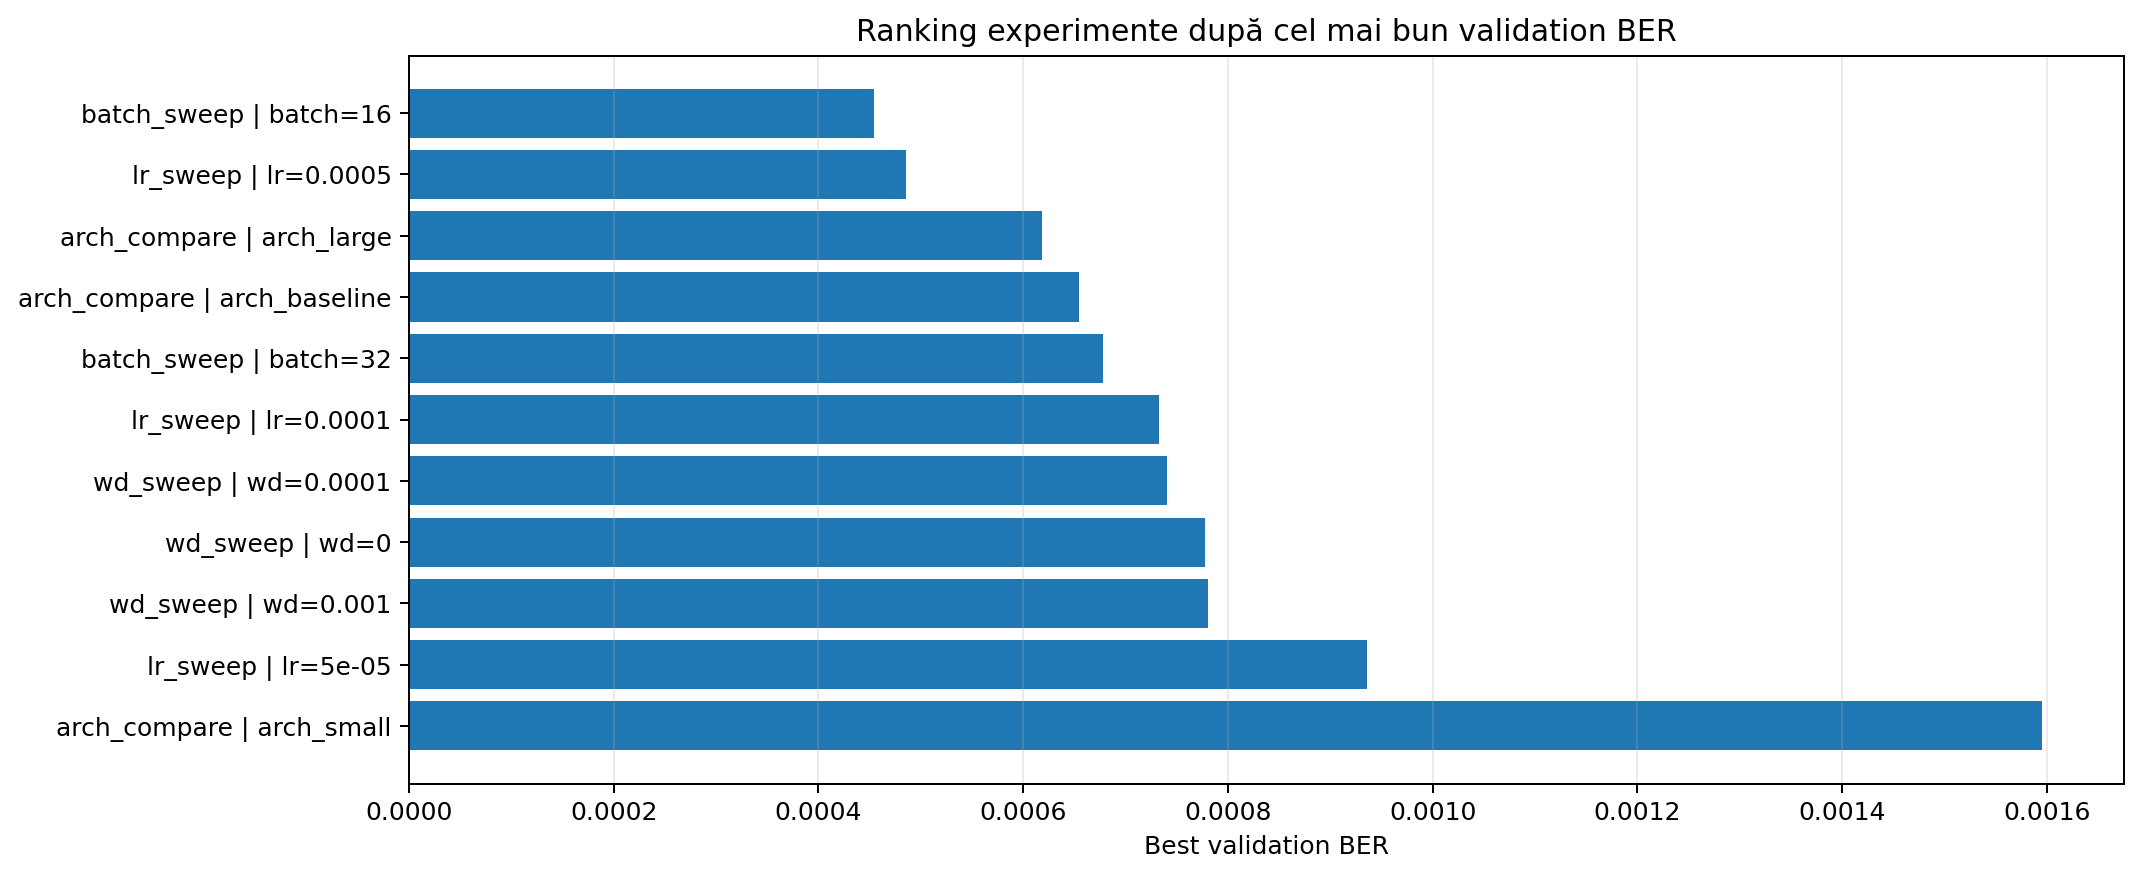
\includegraphics[width=0.9\textwidth]{images/08_ranking_best_val_ber.png}
    \caption{Clasamentul experimentelor după cel mai bun BER obținut pe setul de validare}
\end{figure}
\FloatBarrier

\begin{figure}[htbp]
    \centering
    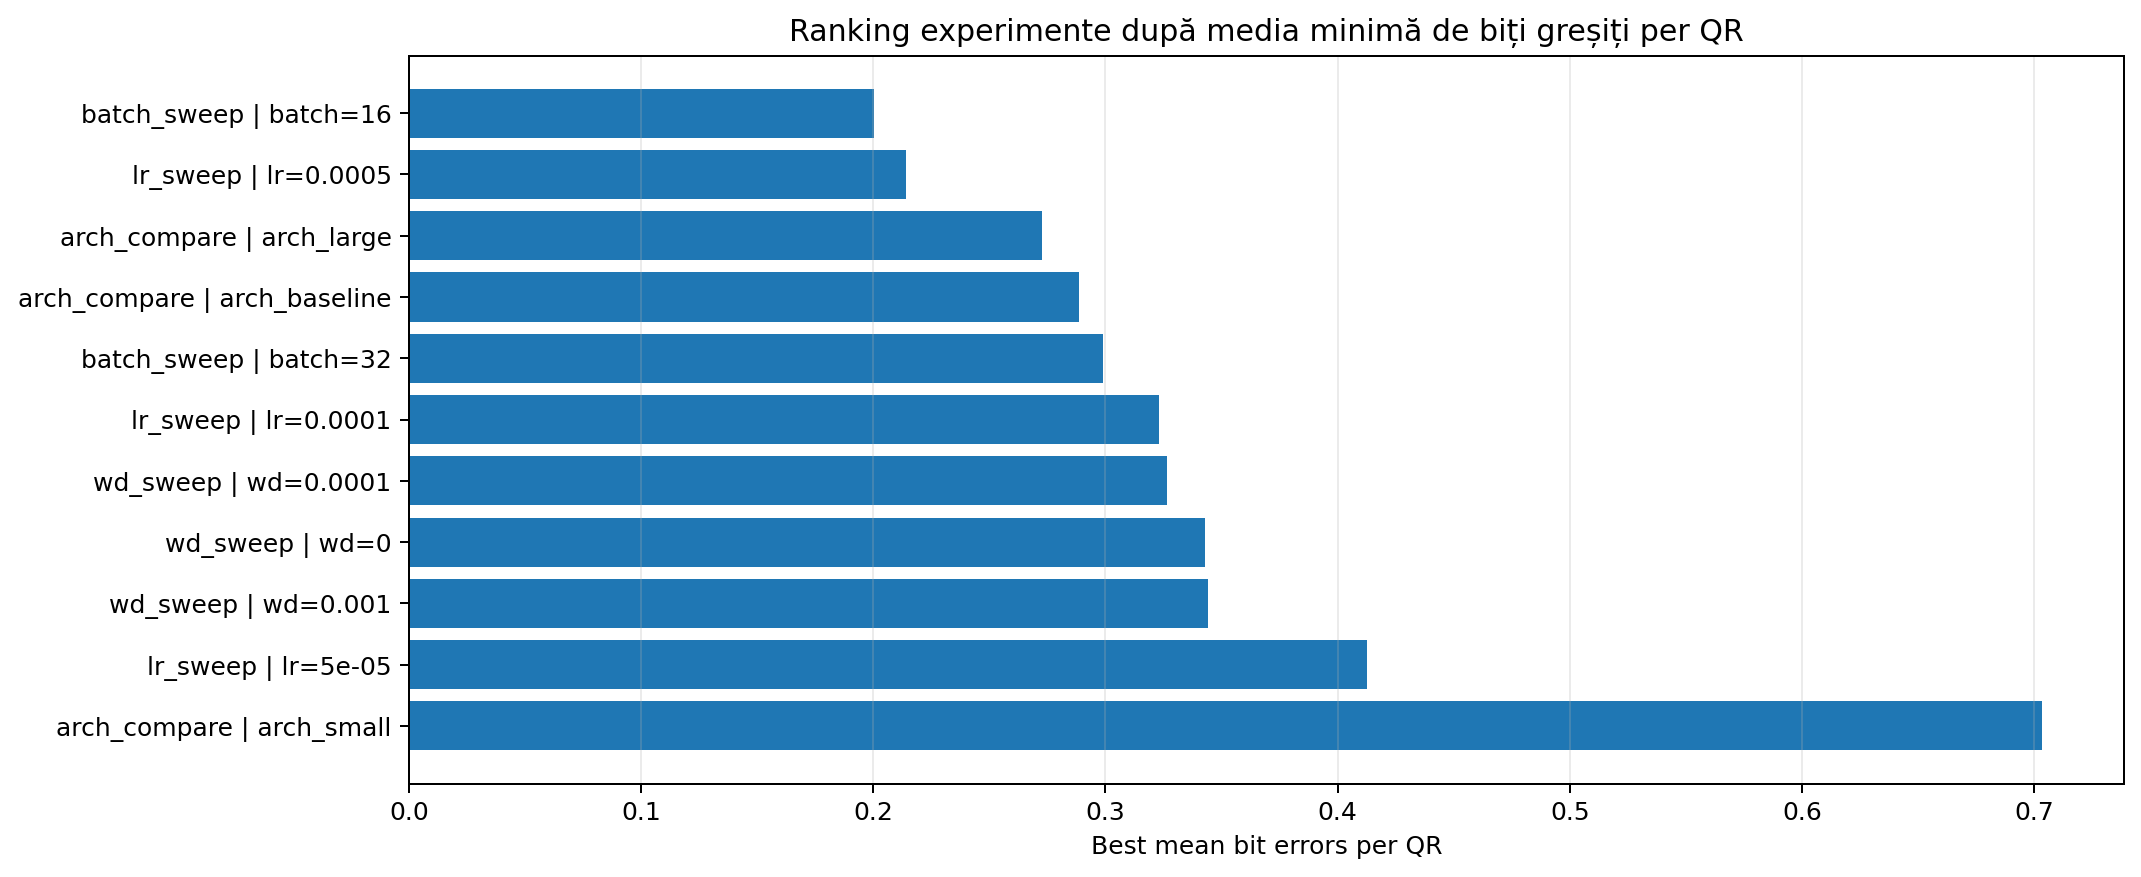
\includegraphics[width=0.9\textwidth]{images/09_ranking_best_mean_bit_errors_per_qr.png}
    \caption{Clasamentul experimentelor după numărul mediu minim de erori pe cod QR}
\end{figure}
\FloatBarrier

În analiza dimensiunii batch-ului, batch size $16$ a obținut cel mai bun rezultat. Comparativ cu batch size $32$, acesta a redus cel mai bun $val\_ber$ de la $0.000678$ la $0.000455$. De asemenea, numărul mediu de erori pe cod QR a scăzut de la $0.2990$ la $0.2005$.

\[
    BER_{batch=16} = 0.000455
\]

\[
    BER_{batch=32} = 0.000678
\]

Această diferență sugerează că batch-ul mai mic a oferit o generalizare ușor mai bună pentru această problemă. În același timp, batch size $16$ a avut și un timp total de training mai mic, de $92.75$ minute, comparativ cu $117.49$ minute pentru batch size $32$.

\begin{figure}[htbp]
    \centering
    \begin{minipage}{0.48\textwidth}
        \centering
        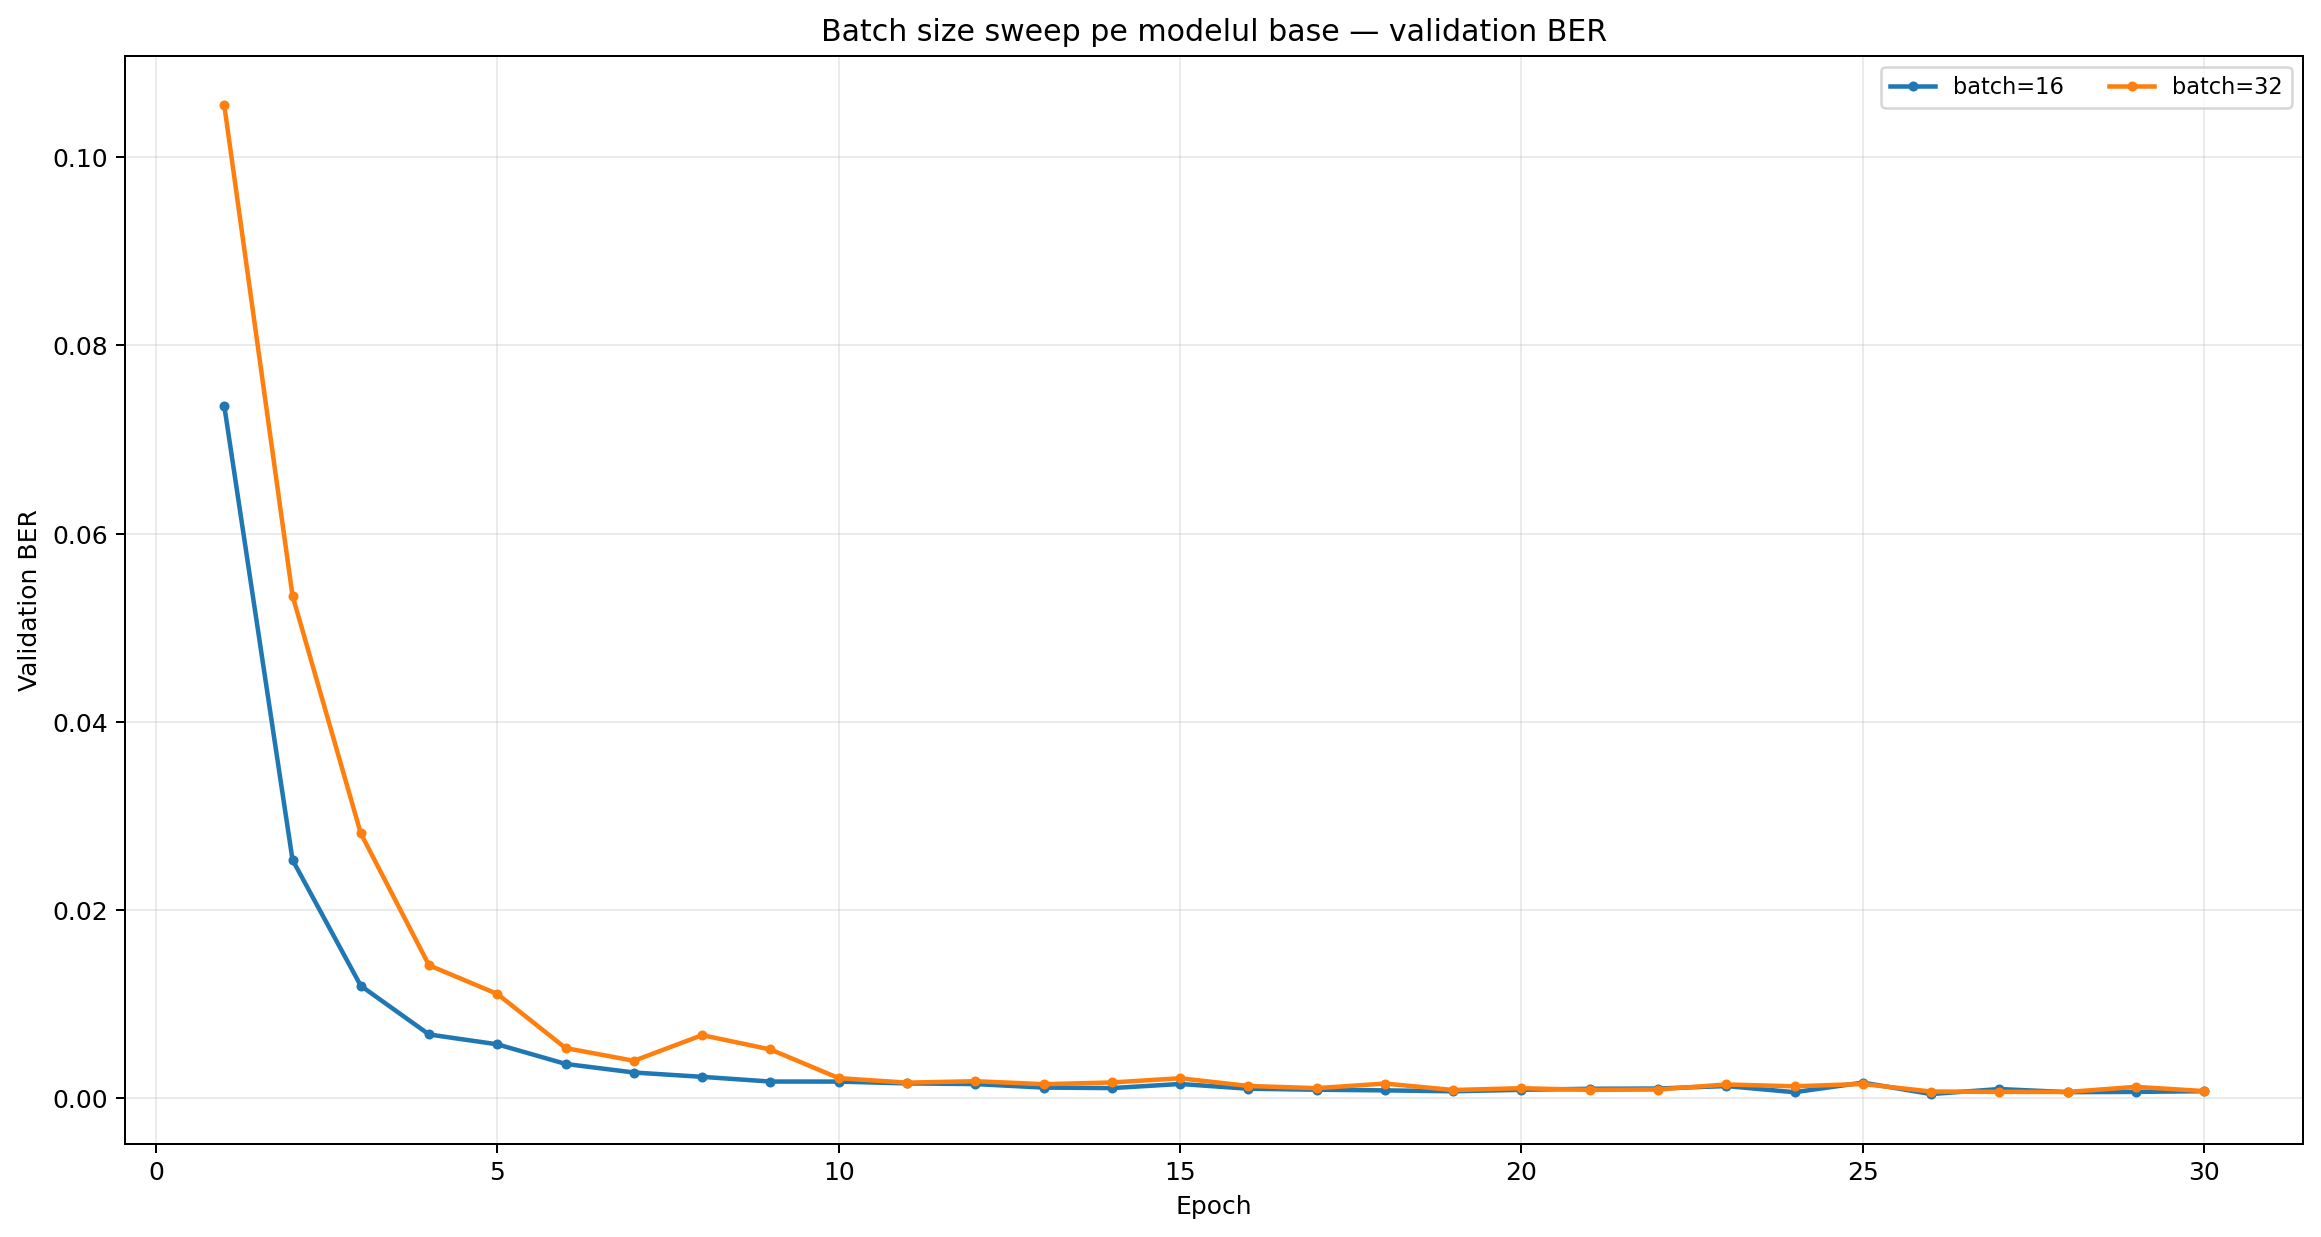
\includegraphics[width=1\textwidth]{images/05_batch-sweep_val_ber_by_epoch.png}
        \caption{Influența dimensiunii batch-ului asupra BER-ului pe validare}
    \end{minipage}
    \hspace{0.03\textwidth}
    \begin{minipage}{0.48\textwidth}
        \centering
        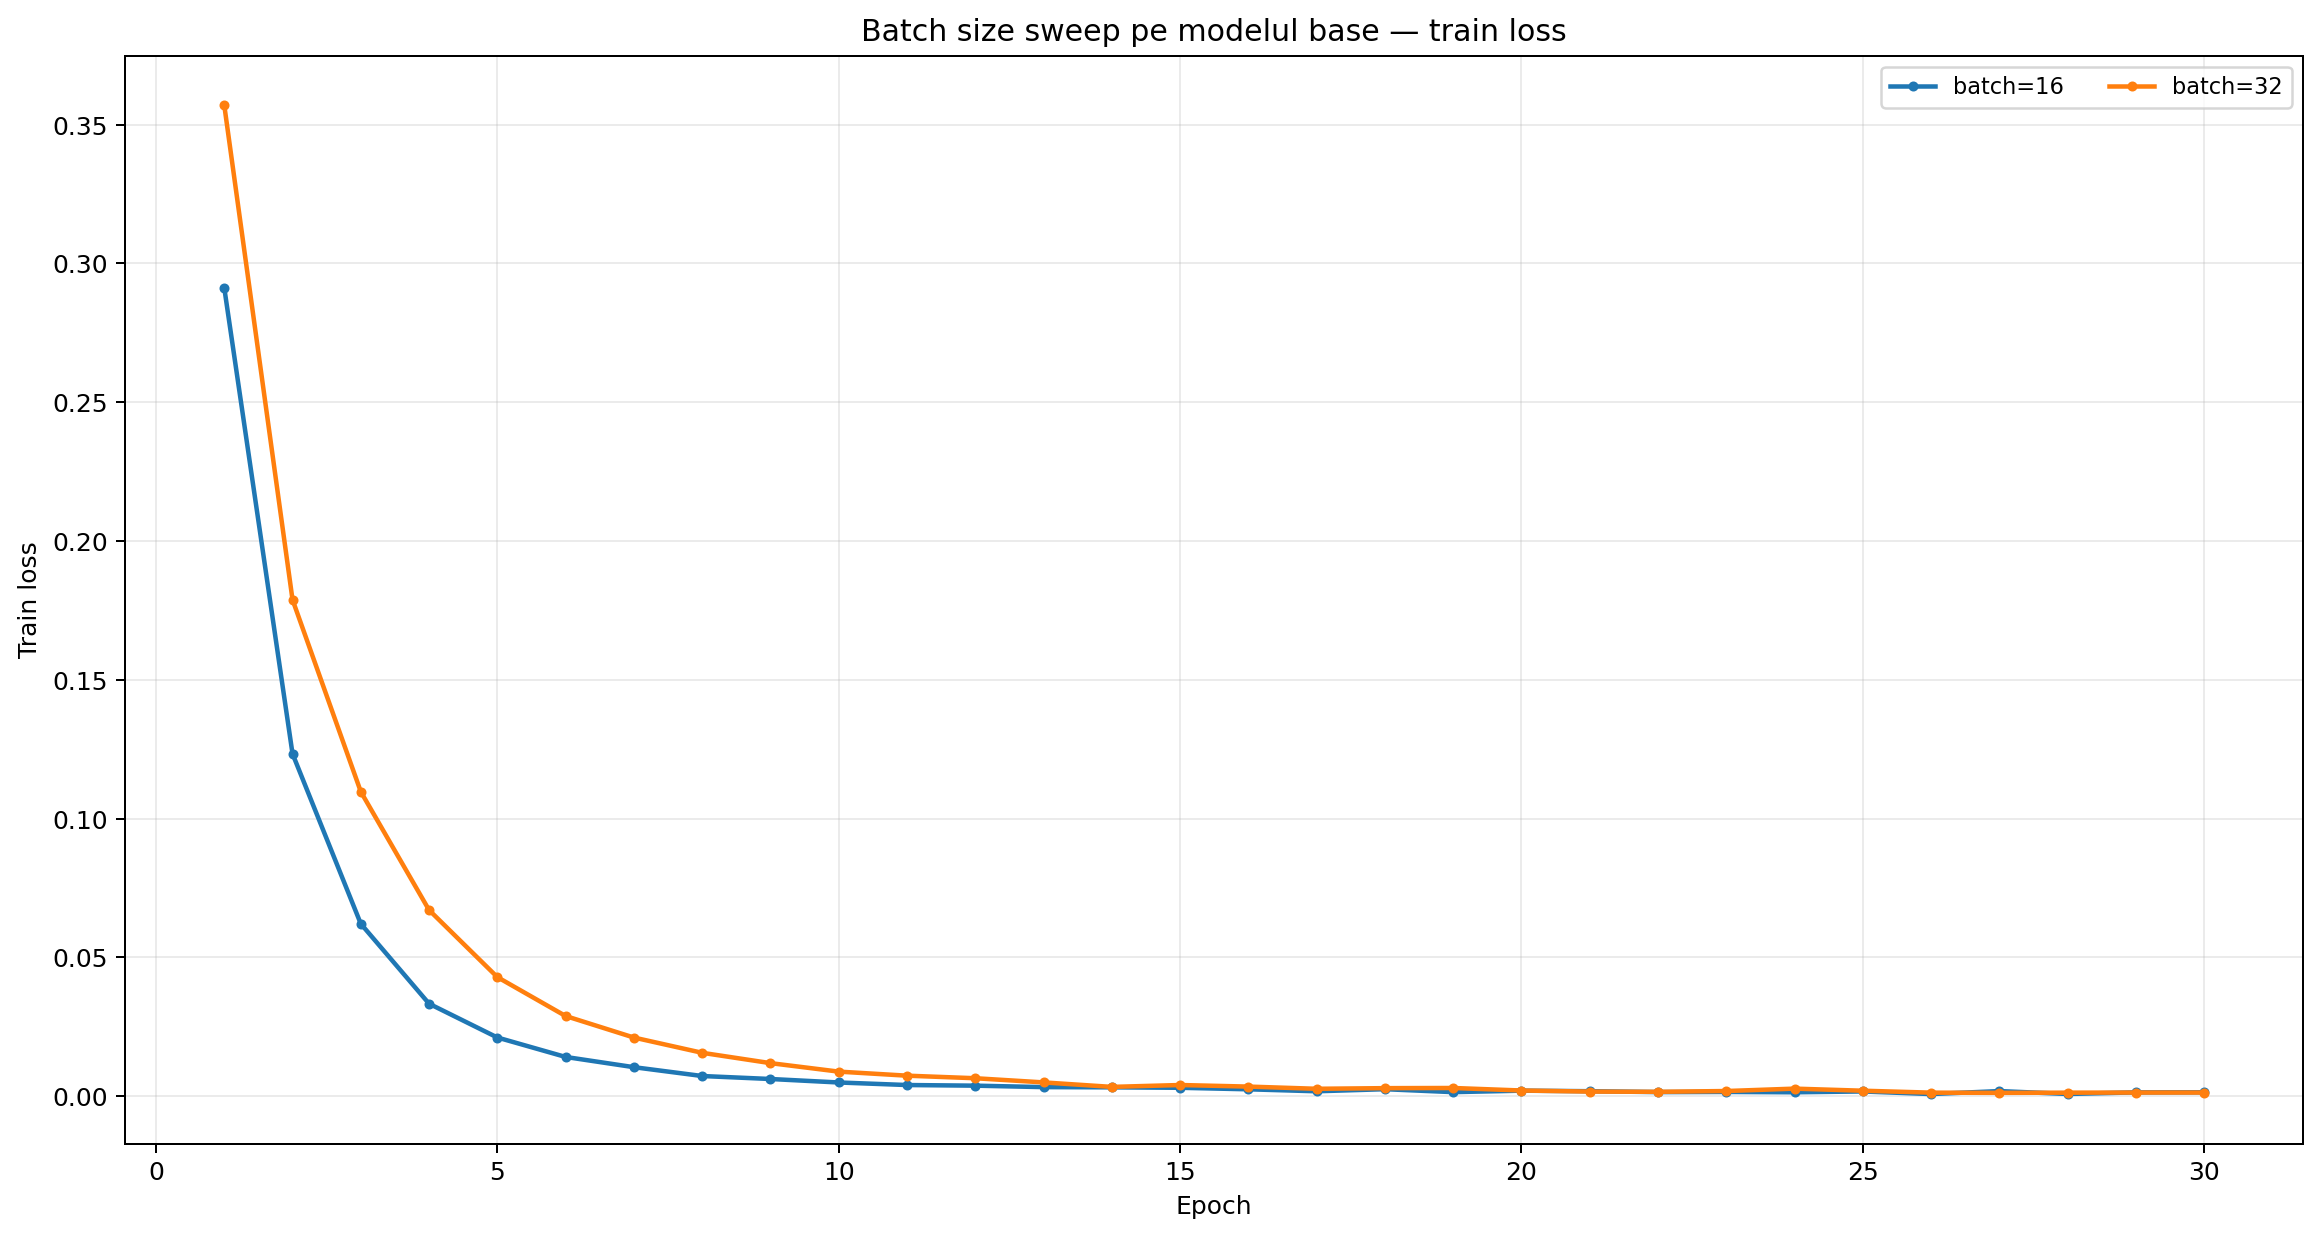
\includegraphics[width=1\textwidth]{images/06_batch-sweep_train_loss_by_epoch.png}
        \caption{Influența dimensiunii batch-ului asupra pierderii pe antrenare}
    \end{minipage}
\end{figure}
\FloatBarrier

În analiza ratei de învățare, cea mai bună valoare a fost $5 \cdot 10^{-4}$. Această configurație a obținut un $val\_ber$ minim de $0.000485$, foarte apropiat de cel mai bun rezultat global. Rata de învățare $10^{-4}$ a obținut $0.000732$, iar rata de învățare $5 \cdot 10^{-5}$ a obținut $0.000935$.

\[
    BER_{lr=5 \cdot 10^{-4}} = 0.000485
\]

\[
    BER_{lr=10^{-4}} = 0.000732
\]

\[
    BER_{lr=5 \cdot 10^{-5}} = 0.000935
\]

Rezultatele indică faptul că rata de învățare mai mare a accelerat convergența și a permis obținerea unei erori mai mici pe setul de validare. Totuși, configurația cu $lr = 5 \cdot 10^{-4}$ a avut o pierdere finală pe antrenare mai mare decât alte configurații, ceea ce sugerează un comportament mai puțin stabil în ultimele epoci, chiar dacă performanța pe validare a fost foarte bună.

\begin{figure}[htbp]
    \centering
    \begin{minipage}{0.48\textwidth}
        \centering
        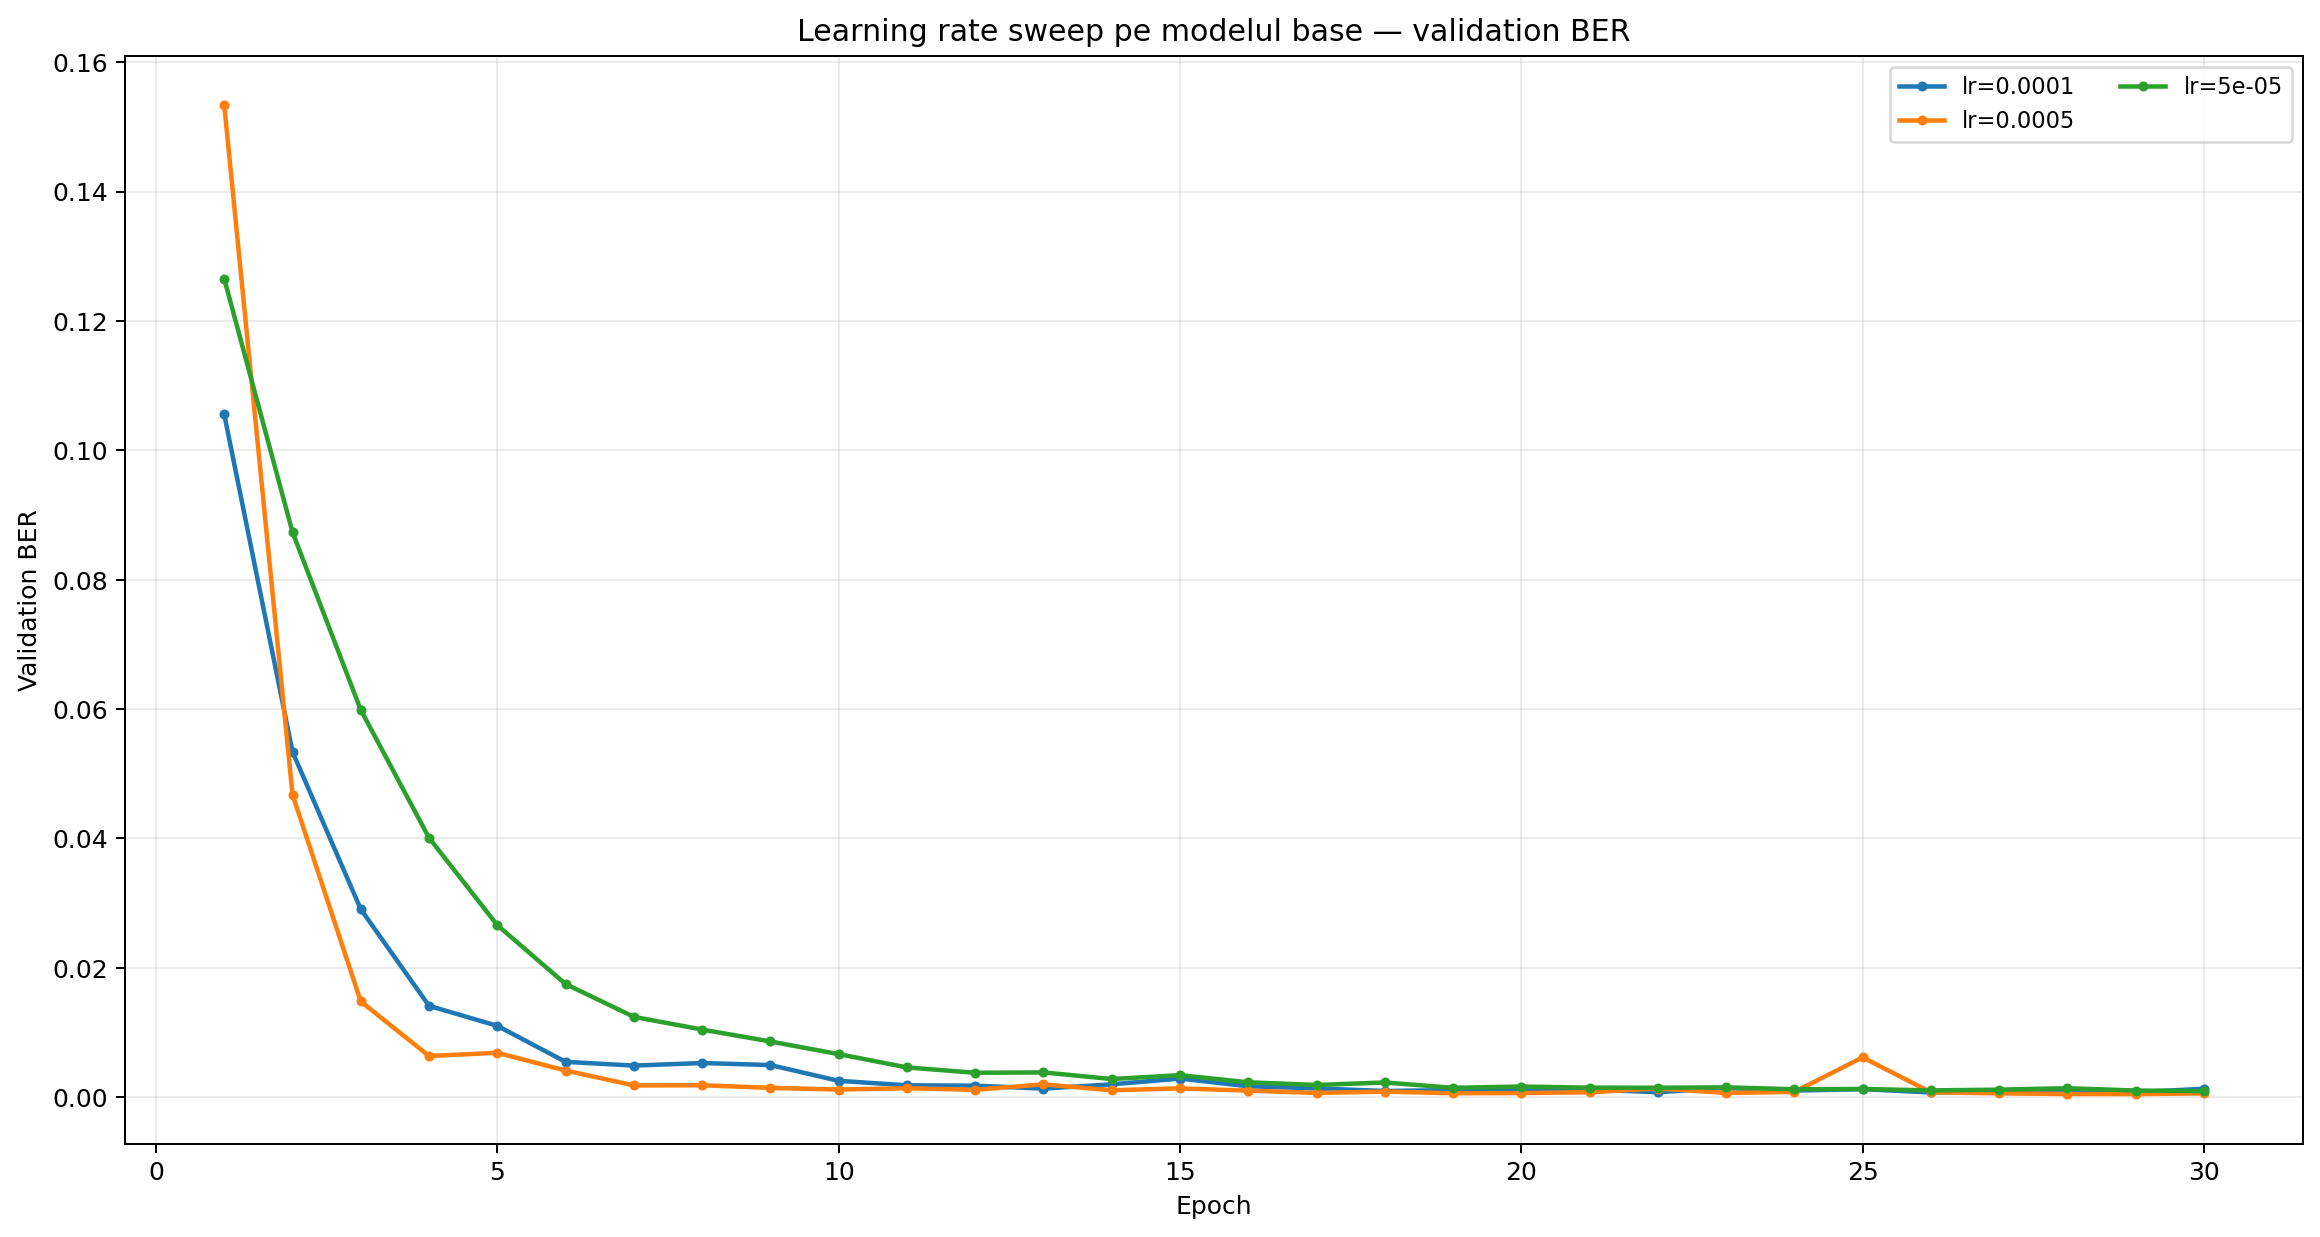
\includegraphics[width=1\textwidth]{images/05_lr-sweep_val_ber_by_epoch.png}
        \caption{Influența ratei de învățare asupra BER-ului pe validare}
    \end{minipage}
    \hspace{0.03\textwidth}
    \begin{minipage}{0.48\textwidth}
        \centering
        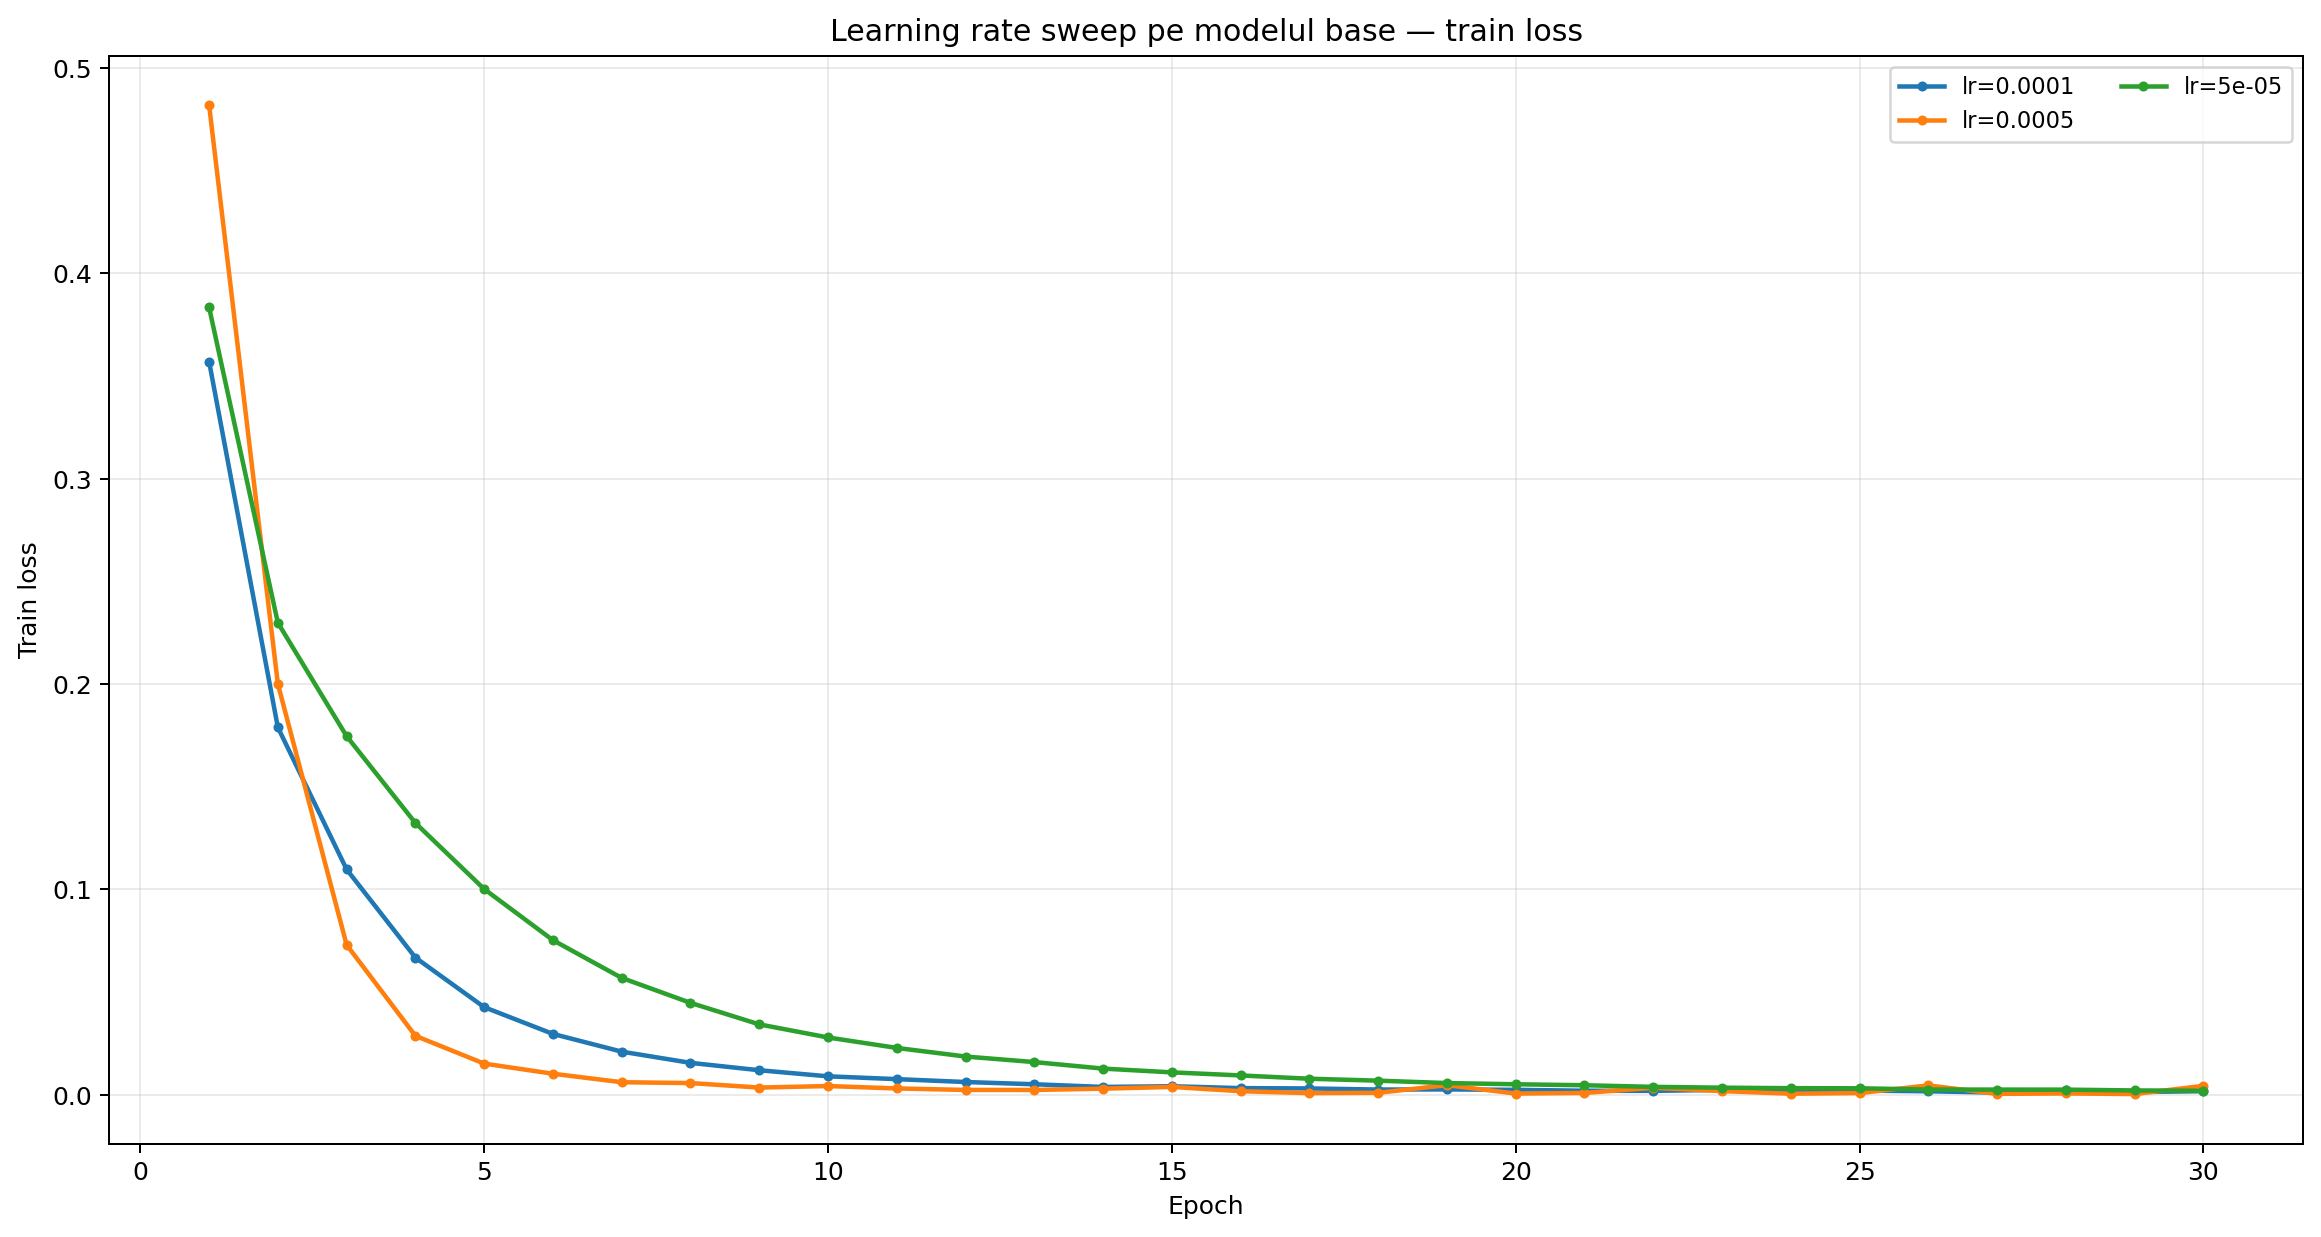
\includegraphics[width=1\textwidth]{images/06_lr-sweep_train_loss_by_epoch.png}
        \caption{Influența ratei de învățare asupra pierderii pe antrenare}
    \end{minipage}
\end{figure}
\FloatBarrier

În analiza regularizării, cele trei valori testate pentru weight decay au produs rezultate apropiate. Cea mai bună configurație din această categorie a fost cea cu $weightDecay = 10^{-4}$, care a obținut $val\_ber = 0.000740$. Fără regularizare, modelul a obținut $0.000778$, iar pentru $weightDecay = 10^{-3}$ a obținut $0.000780$.

\[
    BER_{wd=10^{-4}} = 0.000740
\]

\[
    BER_{wd=0} = 0.000778
\]

\[
    BER_{wd=10^{-3}} = 0.000780
\]

Diferențele sunt mici, ceea ce arată că modelul nu este extrem de sensibil la această valoare în intervalul testat. Totuși, regularizarea $10^{-4}$ a oferit cel mai bun compromis în cadrul acestui grup de experimente.

\begin{figure}[htbp]
    \centering
    \begin{minipage}{0.48\textwidth}
        \centering
        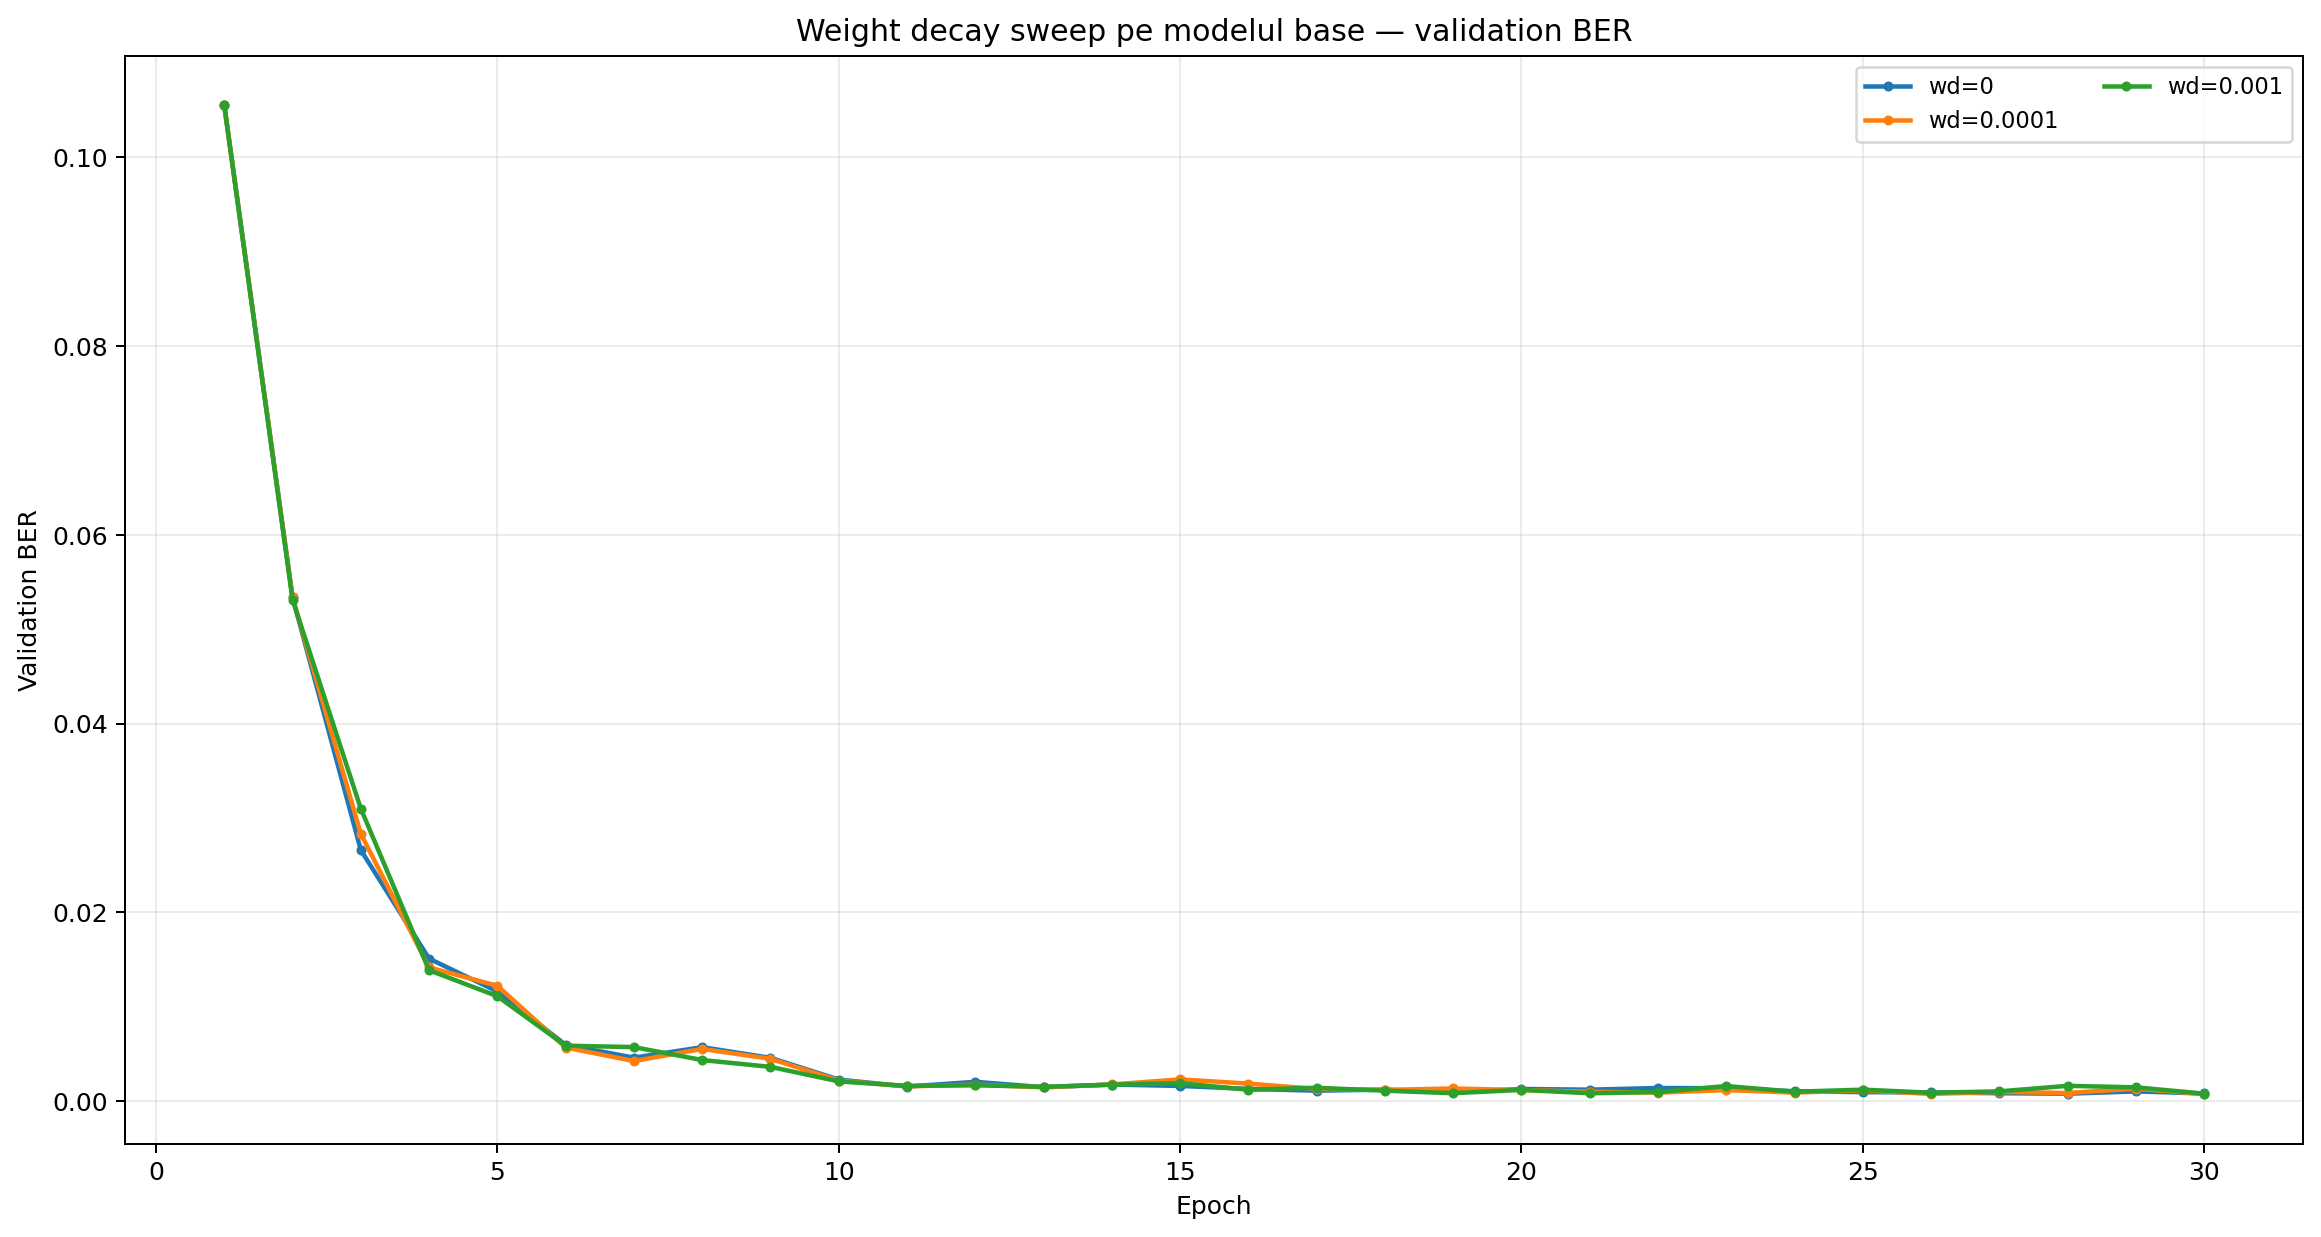
\includegraphics[width=1\textwidth]{images/05_wd-sweep_val_ber_by_epoch.png}
        \caption{Influența regularizării asupra BER-ului pe validare}
    \end{minipage}
    \hspace{0.03\textwidth}
    \begin{minipage}{0.48\textwidth}
        \centering
        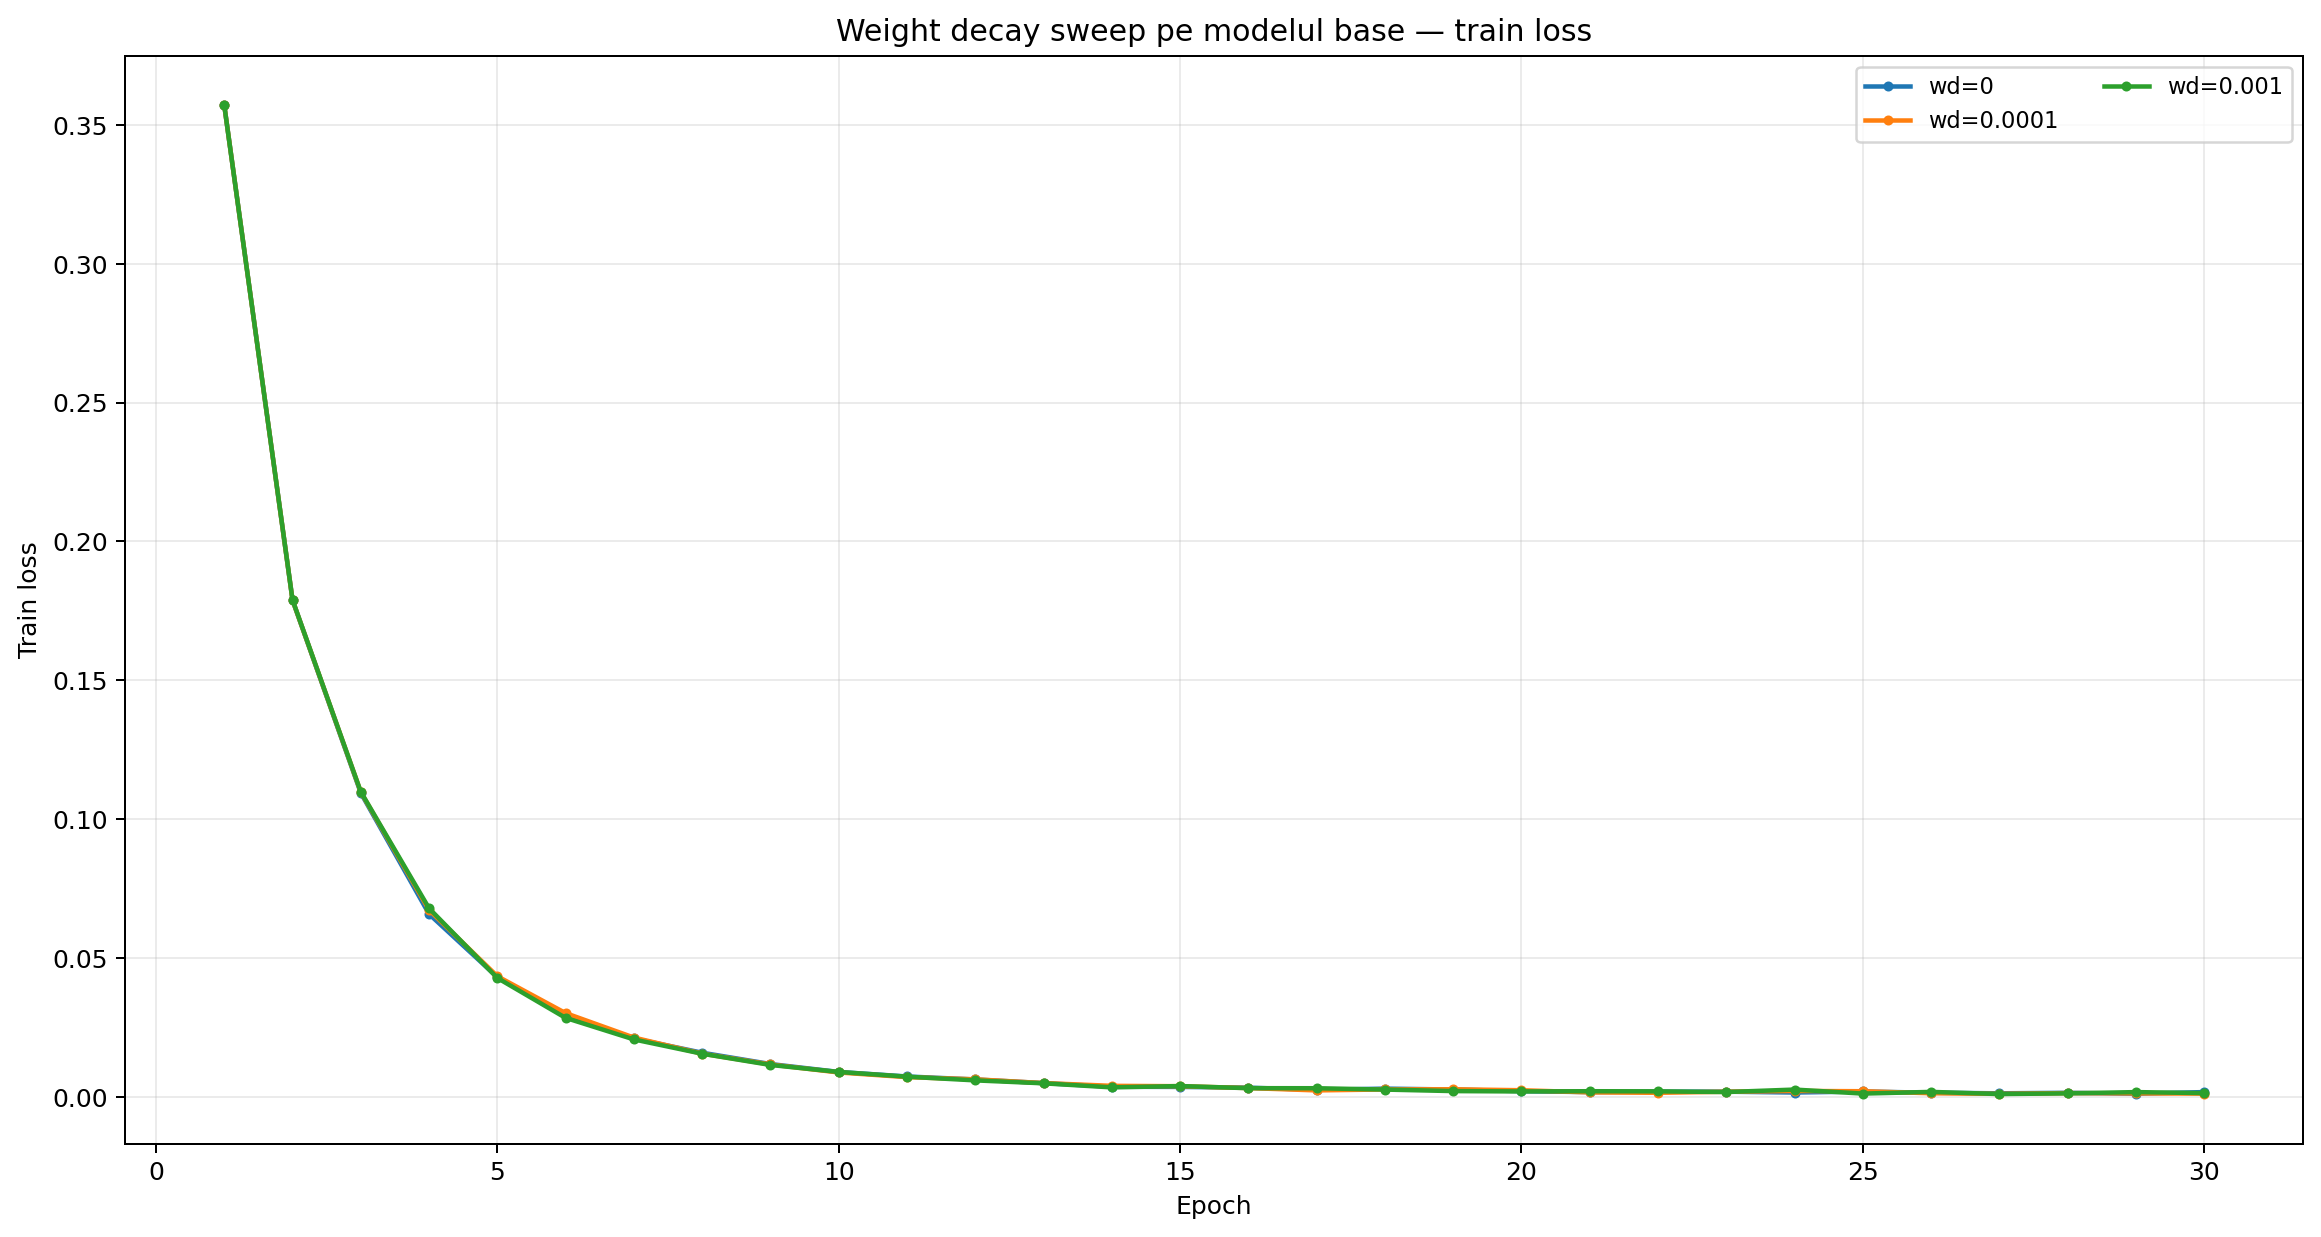
\includegraphics[width=1\textwidth]{images/06_wd-sweep_train_loss_by_epoch.png}
        \caption{Influența regularizării asupra pierderii pe antrenare}
    \end{minipage}
\end{figure}
\FloatBarrier

În comparația arhitecturilor, varianta \textit{arch\_large} a obținut cel mai bun rezultat, cu $val\_ber = 0.000618$. Varianta \textit{arch\_baseline} a fost foarte apropiată, cu $val\_ber = 0.000654$, în timp ce varianta \textit{arch\_small} a obținut $val\_ber = 0.001595$.

\[
    BER_{large} = 0.000618
\]

\[
    BER_{baseline} = 0.000654
\]

\[
    BER_{small} = 0.001595
\]

Rezultatul obținut de arhitectura mare arată că adăugarea de adâncime poate îmbunătăți performanța, dar câștigul față de arhitectura de bază este redus. În schimb, modelul mic are o eroare semnificativ mai mare, deși este mult mai eficient din punct de vedere al timpului de antrenare și al numărului de parametri.

\[
    Parametri_{small} = 546001
\]

\[
    Parametri_{baseline} = 2769313
\]

\[
    Parametri_{large} = 3360161
\]

Modelul \textit{arch\_small} a avut cel mai mic timp mediu pe epocă, egal cu $94.21$ secunde, și cel mai mic timp total de training, egal cu $47.10$ minute. Cu toate acestea, eroarea sa medie a fost de $0.7035$ biți pe cod QR, comparativ cu $0.2005$ biți pentru cel mai bun model global. Astfel, arhitectura mică este avantajoasă ca viteză, dar nu oferă aceeași precizie.

\begin{figure}[htbp]
    \centering
    \begin{minipage}{0.48\textwidth}
        \centering
        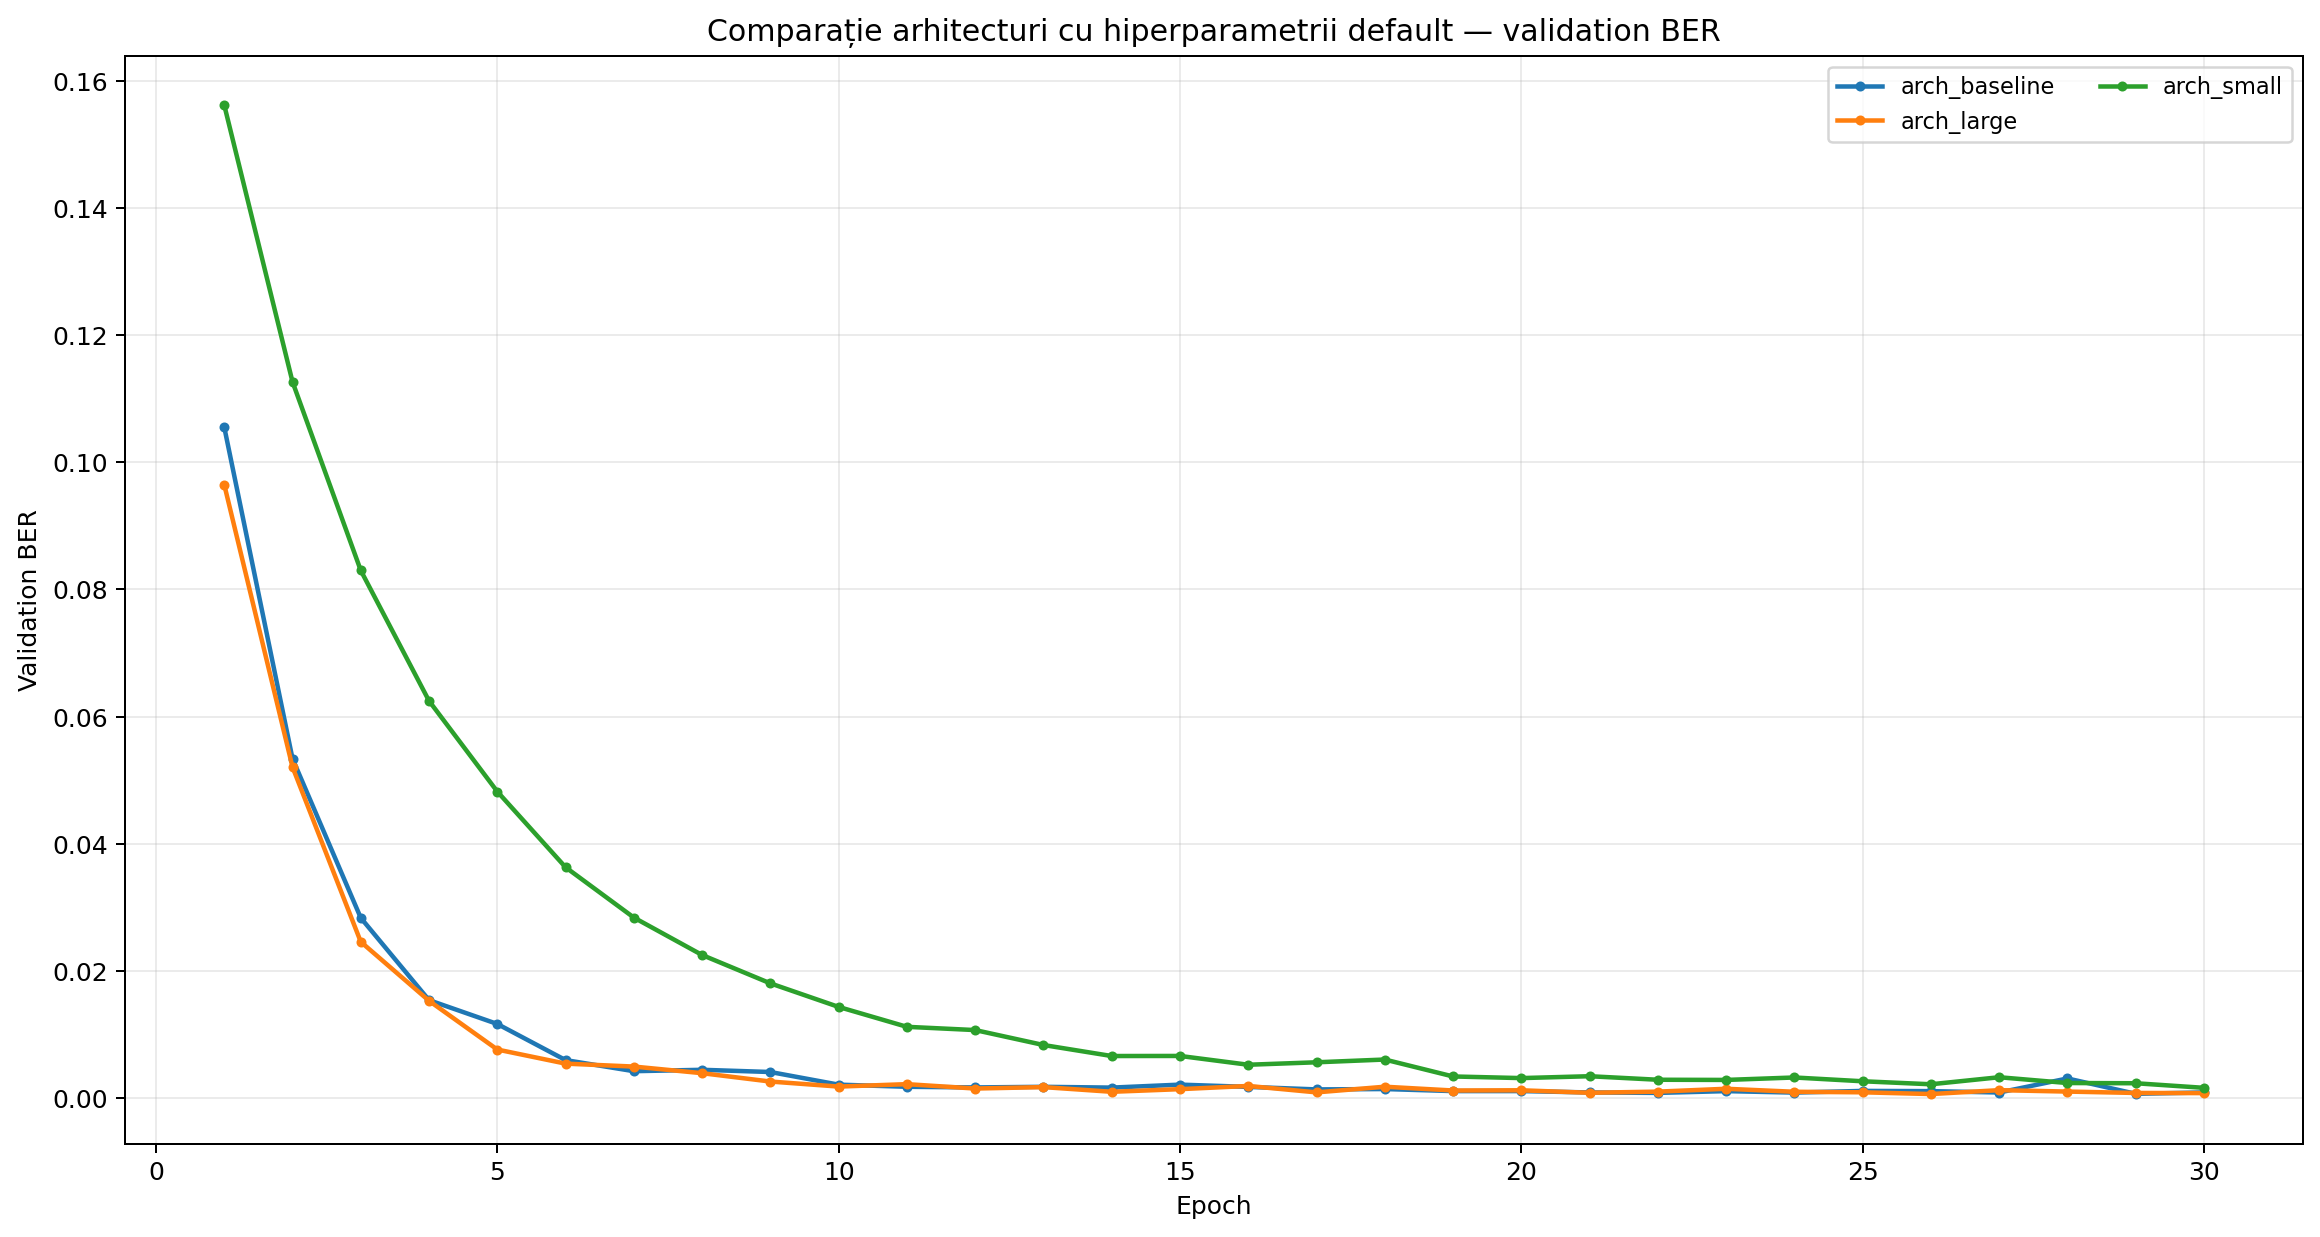
\includegraphics[width=1\textwidth]{images/05_arch-compare_val_ber_by_epoch.png}
        \caption{Comparația arhitecturilor după BER-ul pe validare}
    \end{minipage}
    \hspace{0.03\textwidth}
    \begin{minipage}{0.48\textwidth}
        \centering
        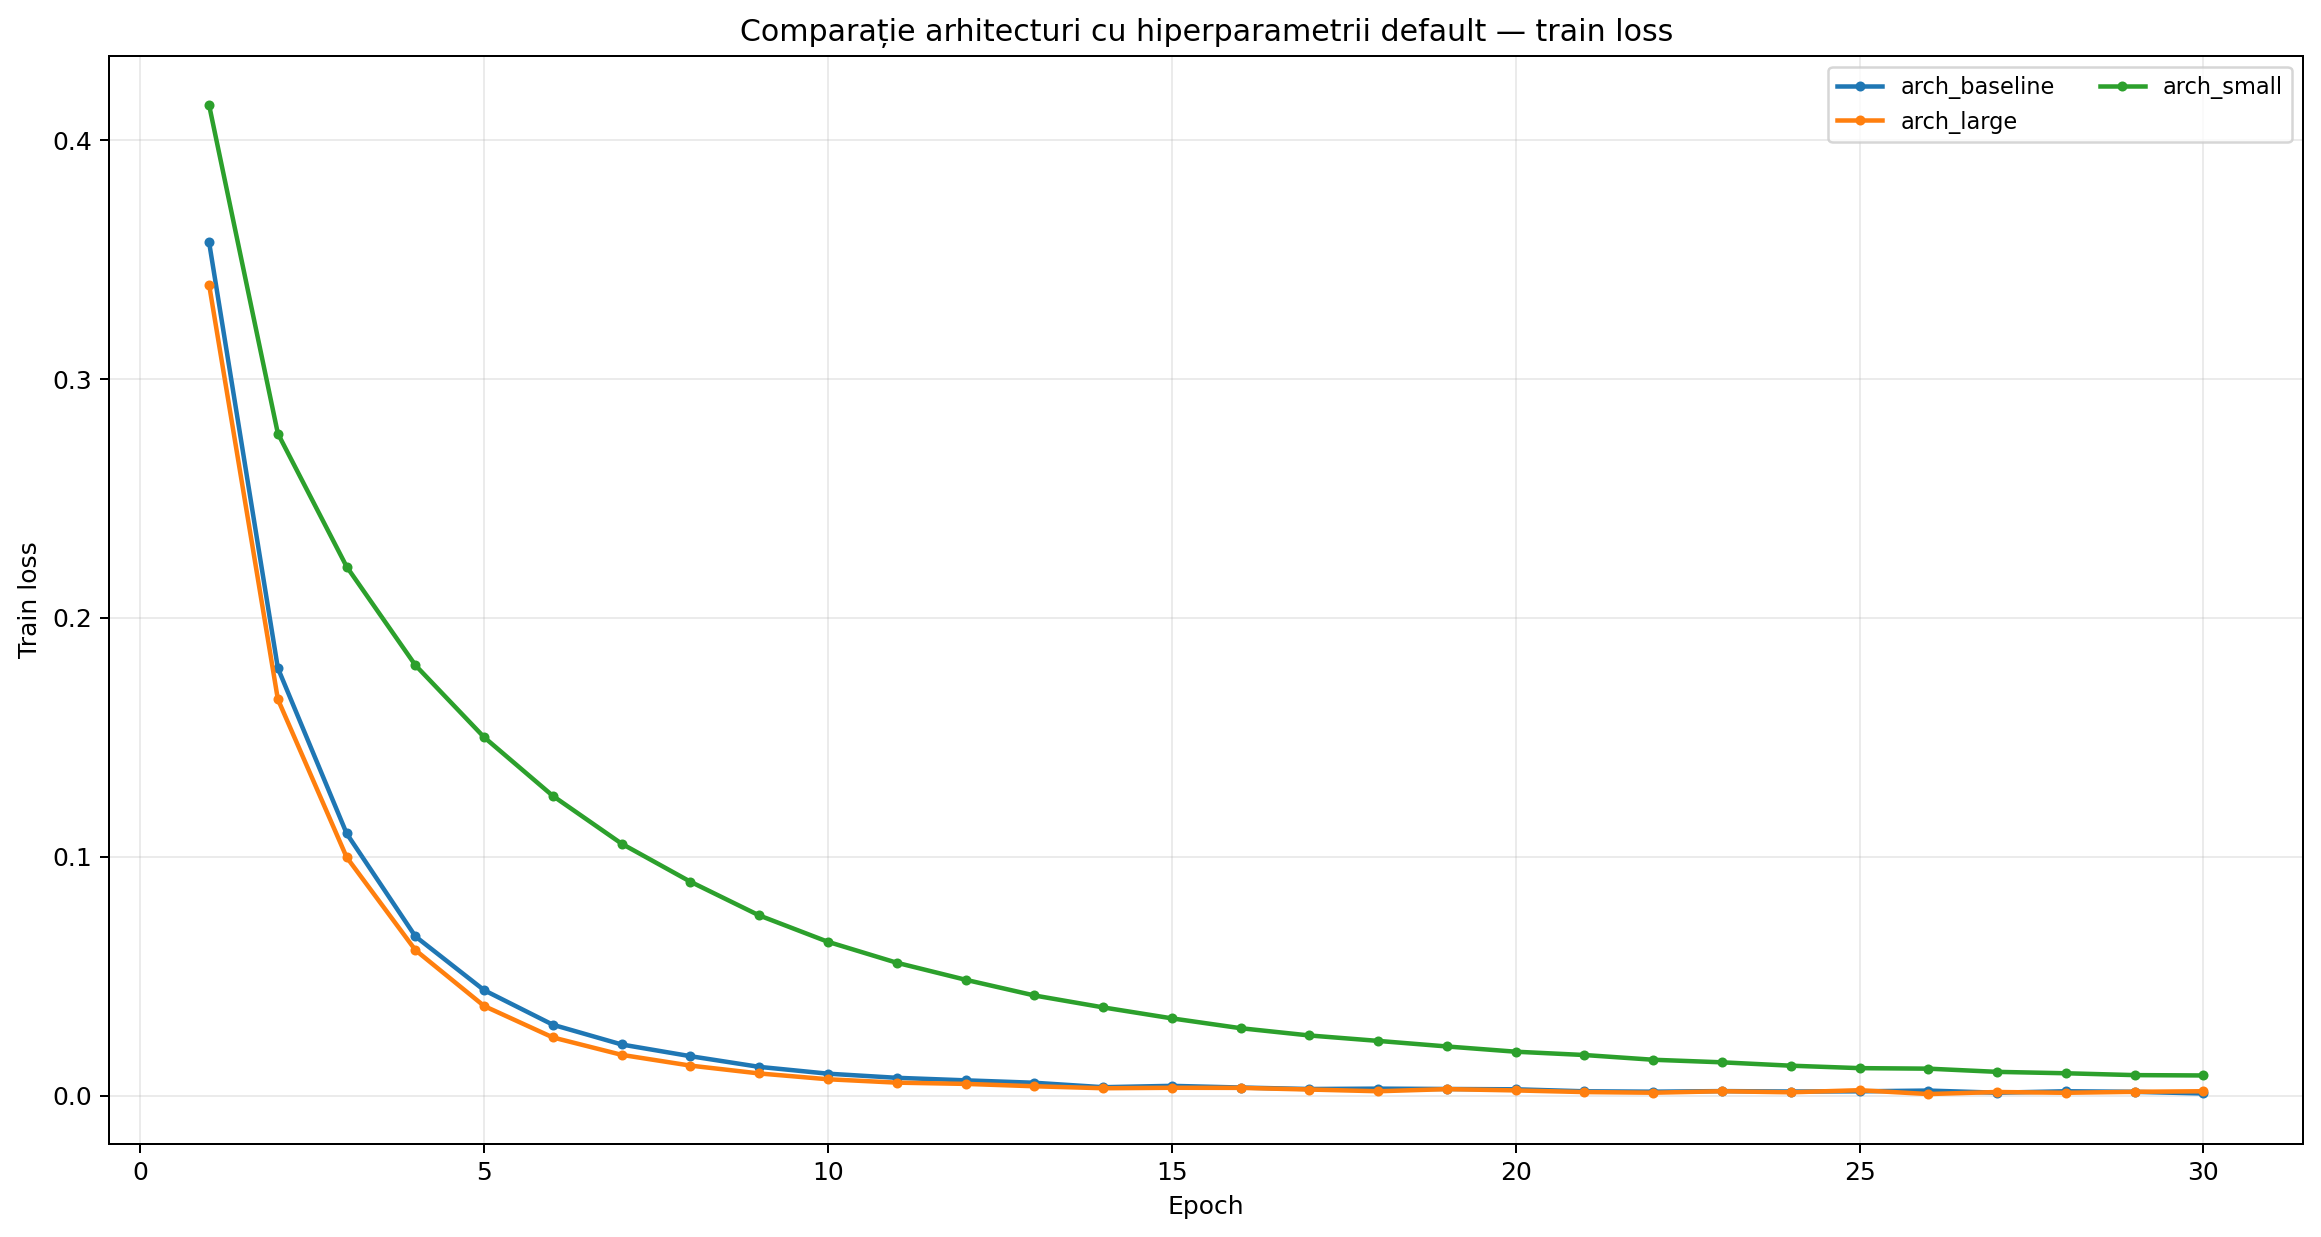
\includegraphics[width=1\textwidth]{images/06_arch-compare_train_loss_by_epoch.png}
        \caption{Comparația arhitecturilor după pierderea pe antrenare}
    \end{minipage}
\end{figure}
\FloatBarrier

Pentru analiza costului de antrenare, au fost urmărite timpul total de training și timpul mediu pe epocă. Cel mai rapid model a fost \textit{arch\_small}, cu $94.21$ secunde pe epocă. Cel mai bun model global, \textit{batch\_sweep\_\_base\_\_batch\_16}, a avut un timp mediu de $185.51$ secunde pe epocă și un timp total de $92.75$ minute. Modelul \textit{arch\_large} a avut un timp mediu de $255.01$ secunde pe epocă și un timp total de $127.50$ minute.

\begin{figure}[htbp]
    \centering
    \begin{minipage}{0.48\textwidth}
        \centering
        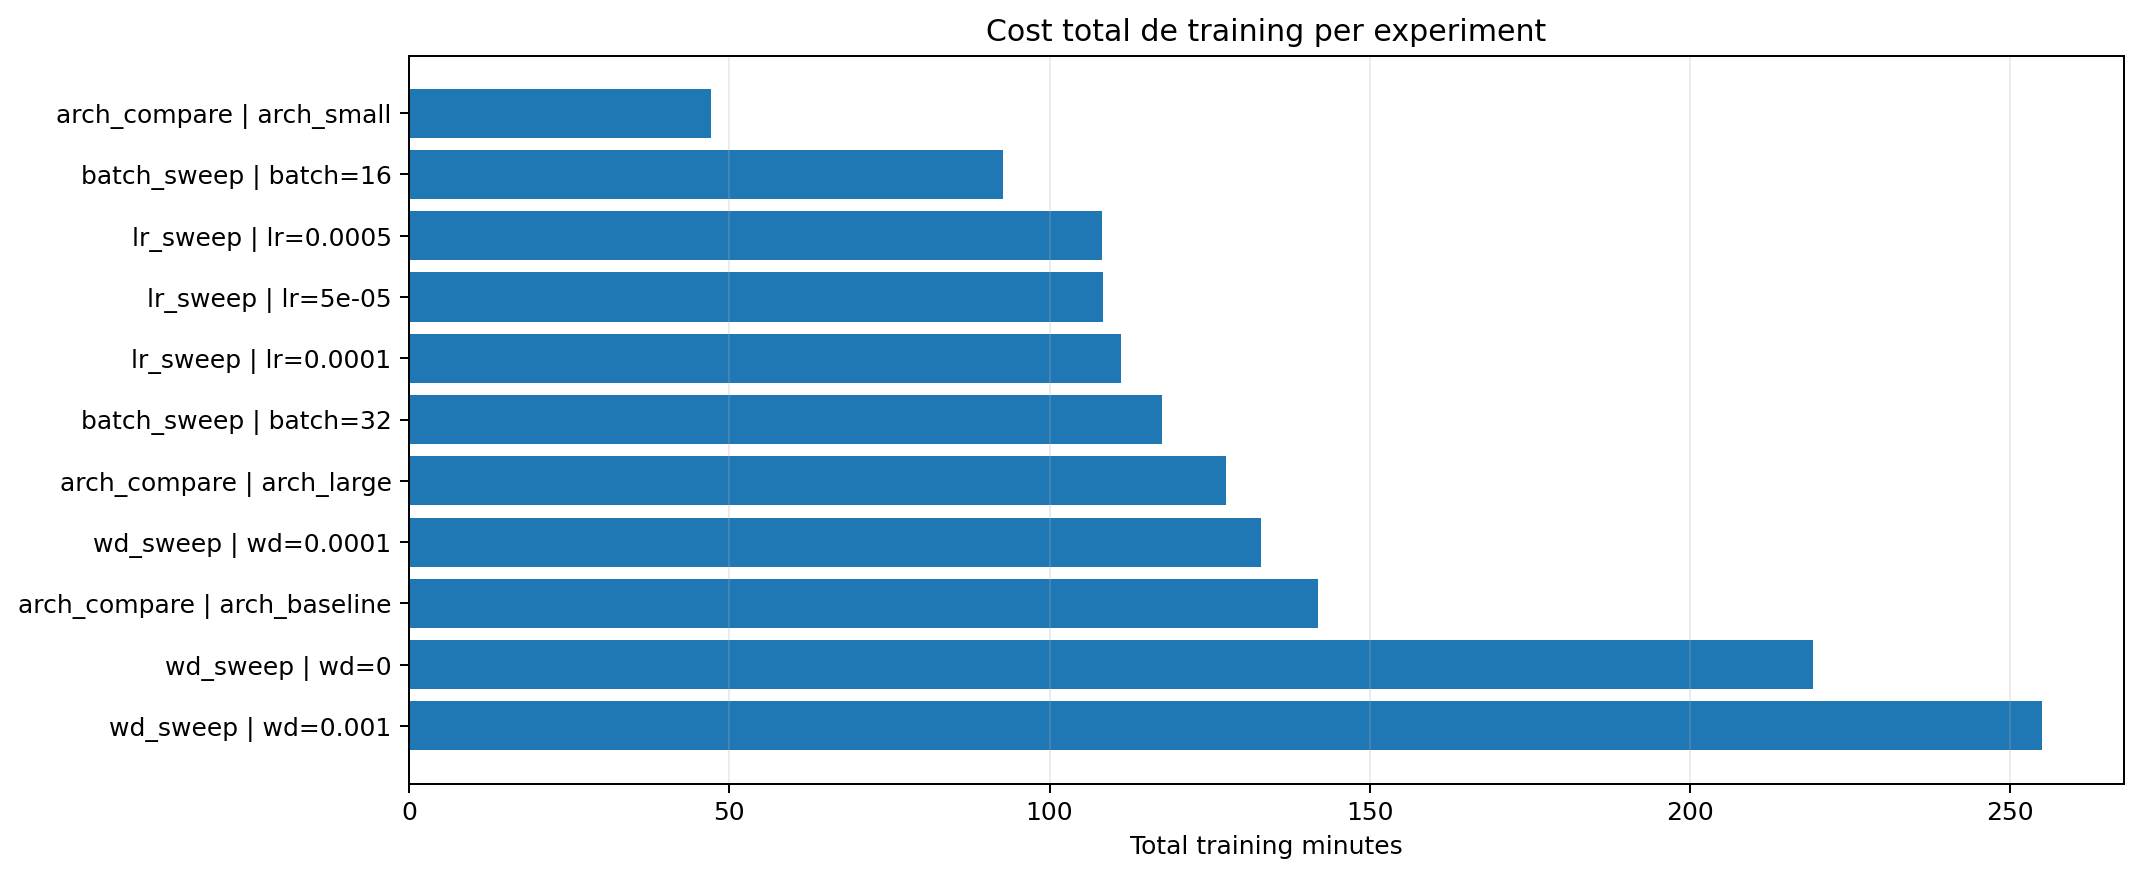
\includegraphics[width=1\textwidth]{images/11_total_training_minutes_by_experiment.png}
        \caption{Timpul total de antrenare pentru fiecare experiment}
    \end{minipage}
    \hspace{0.03\textwidth}
    \begin{minipage}{0.48\textwidth}
        \centering
        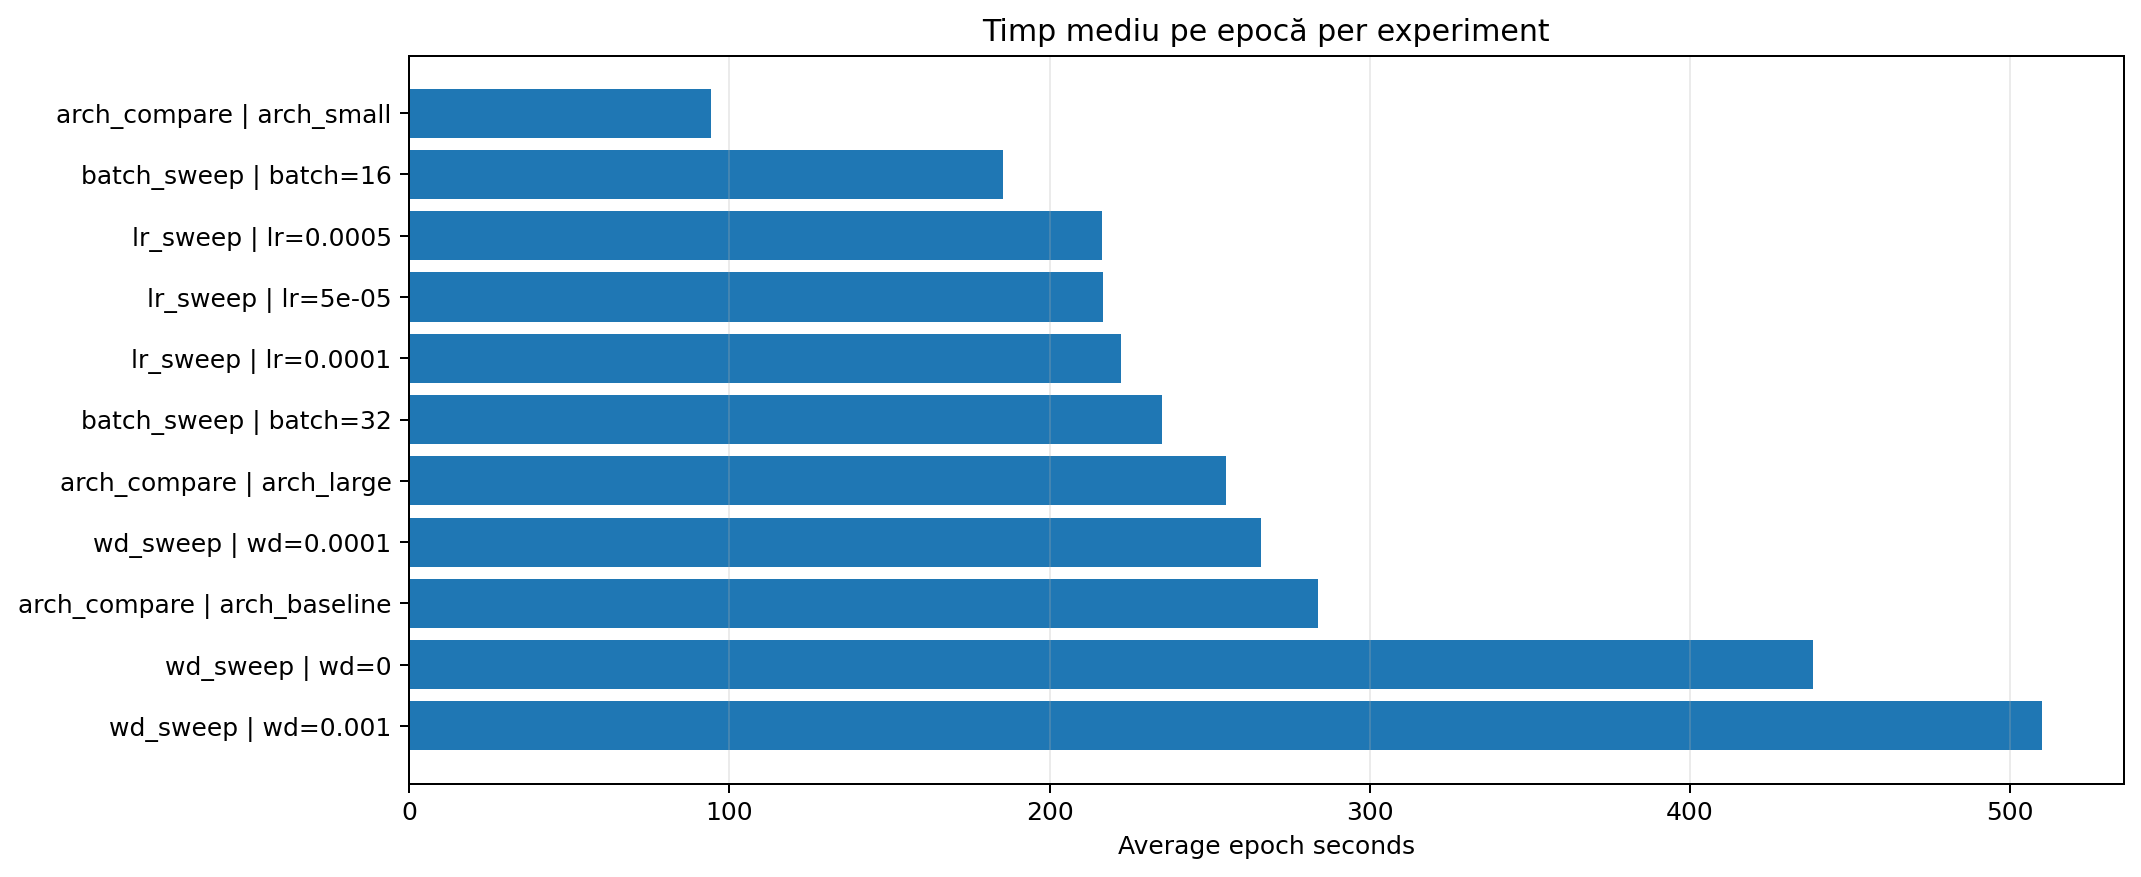
\includegraphics[width=1\textwidth]{images/12_avg_epoch_seconds_by_experiment.png}
        \caption{Timpul mediu pe epocă pentru fiecare experiment}
    \end{minipage}
\end{figure}
\FloatBarrier

Relația dintre performanță și cost poate fi observată mai clar în graficele de tip scatter. Acestea compară cel mai bun $val\_ber$ cu timpul total de antrenare, numărul de parametri și timpul mediu pe epocă. Din aceste grafice se observă că modelul cu batch size $16$ oferă cel mai bun rezultat general, fără a avea cel mai mare cost de antrenare. În schimb, modelul mic este cel mai eficient, dar pierde din precizie, iar modelul mare oferă o îmbunătățire față de baseline, însă cu un cost mai ridicat.

\begin{figure}[htbp]
    \centering
    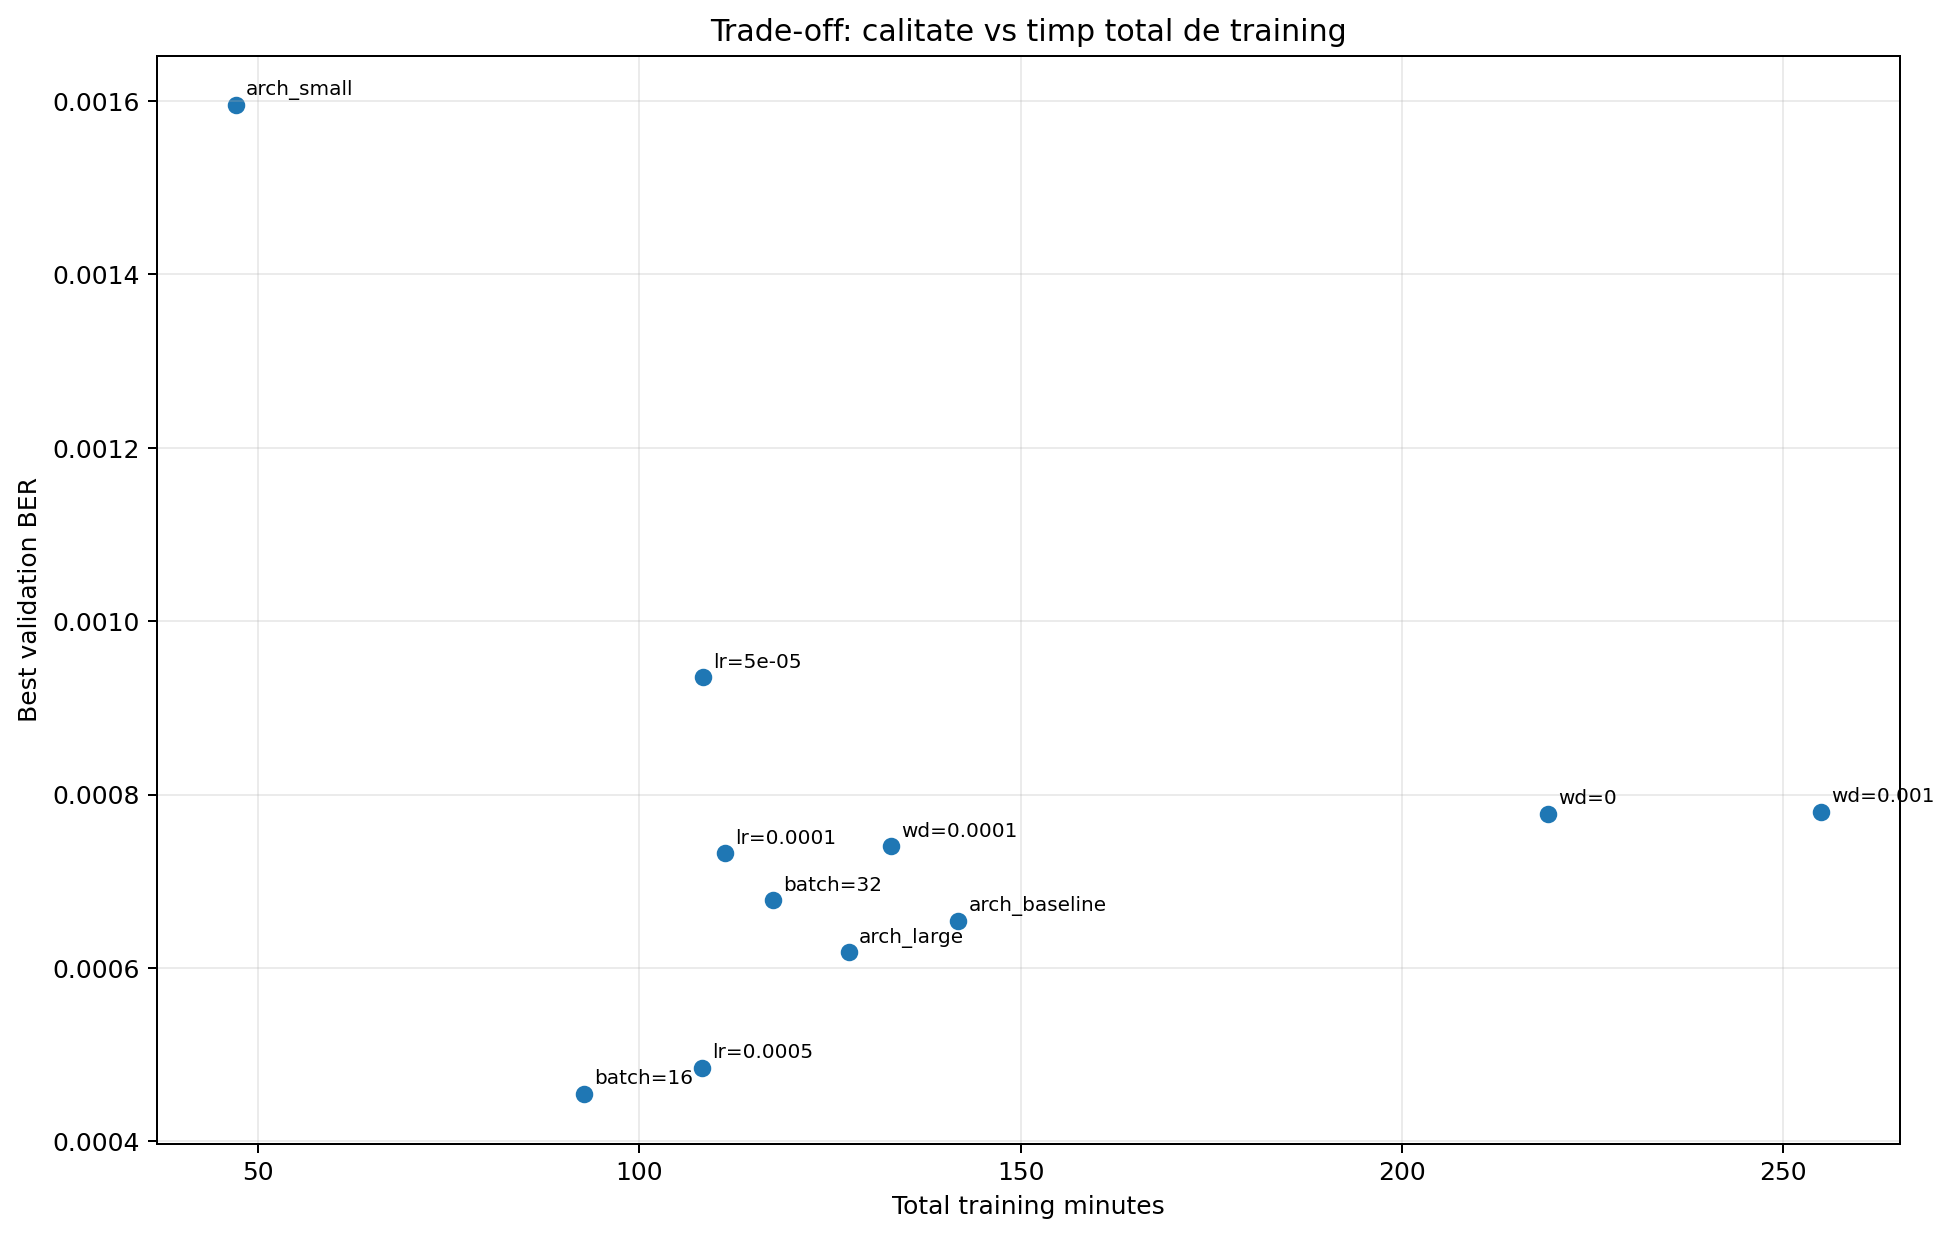
\includegraphics[width=0.75\textwidth]{images/13_scatter_best_val_ber_vs_total_training_minutes.png}
    \caption{Relația dintre BER-ul minim și timpul total de antrenare}
\end{figure}
\FloatBarrier

\begin{figure}[htbp]
    \centering
    \begin{minipage}{0.48\textwidth}
        \centering
        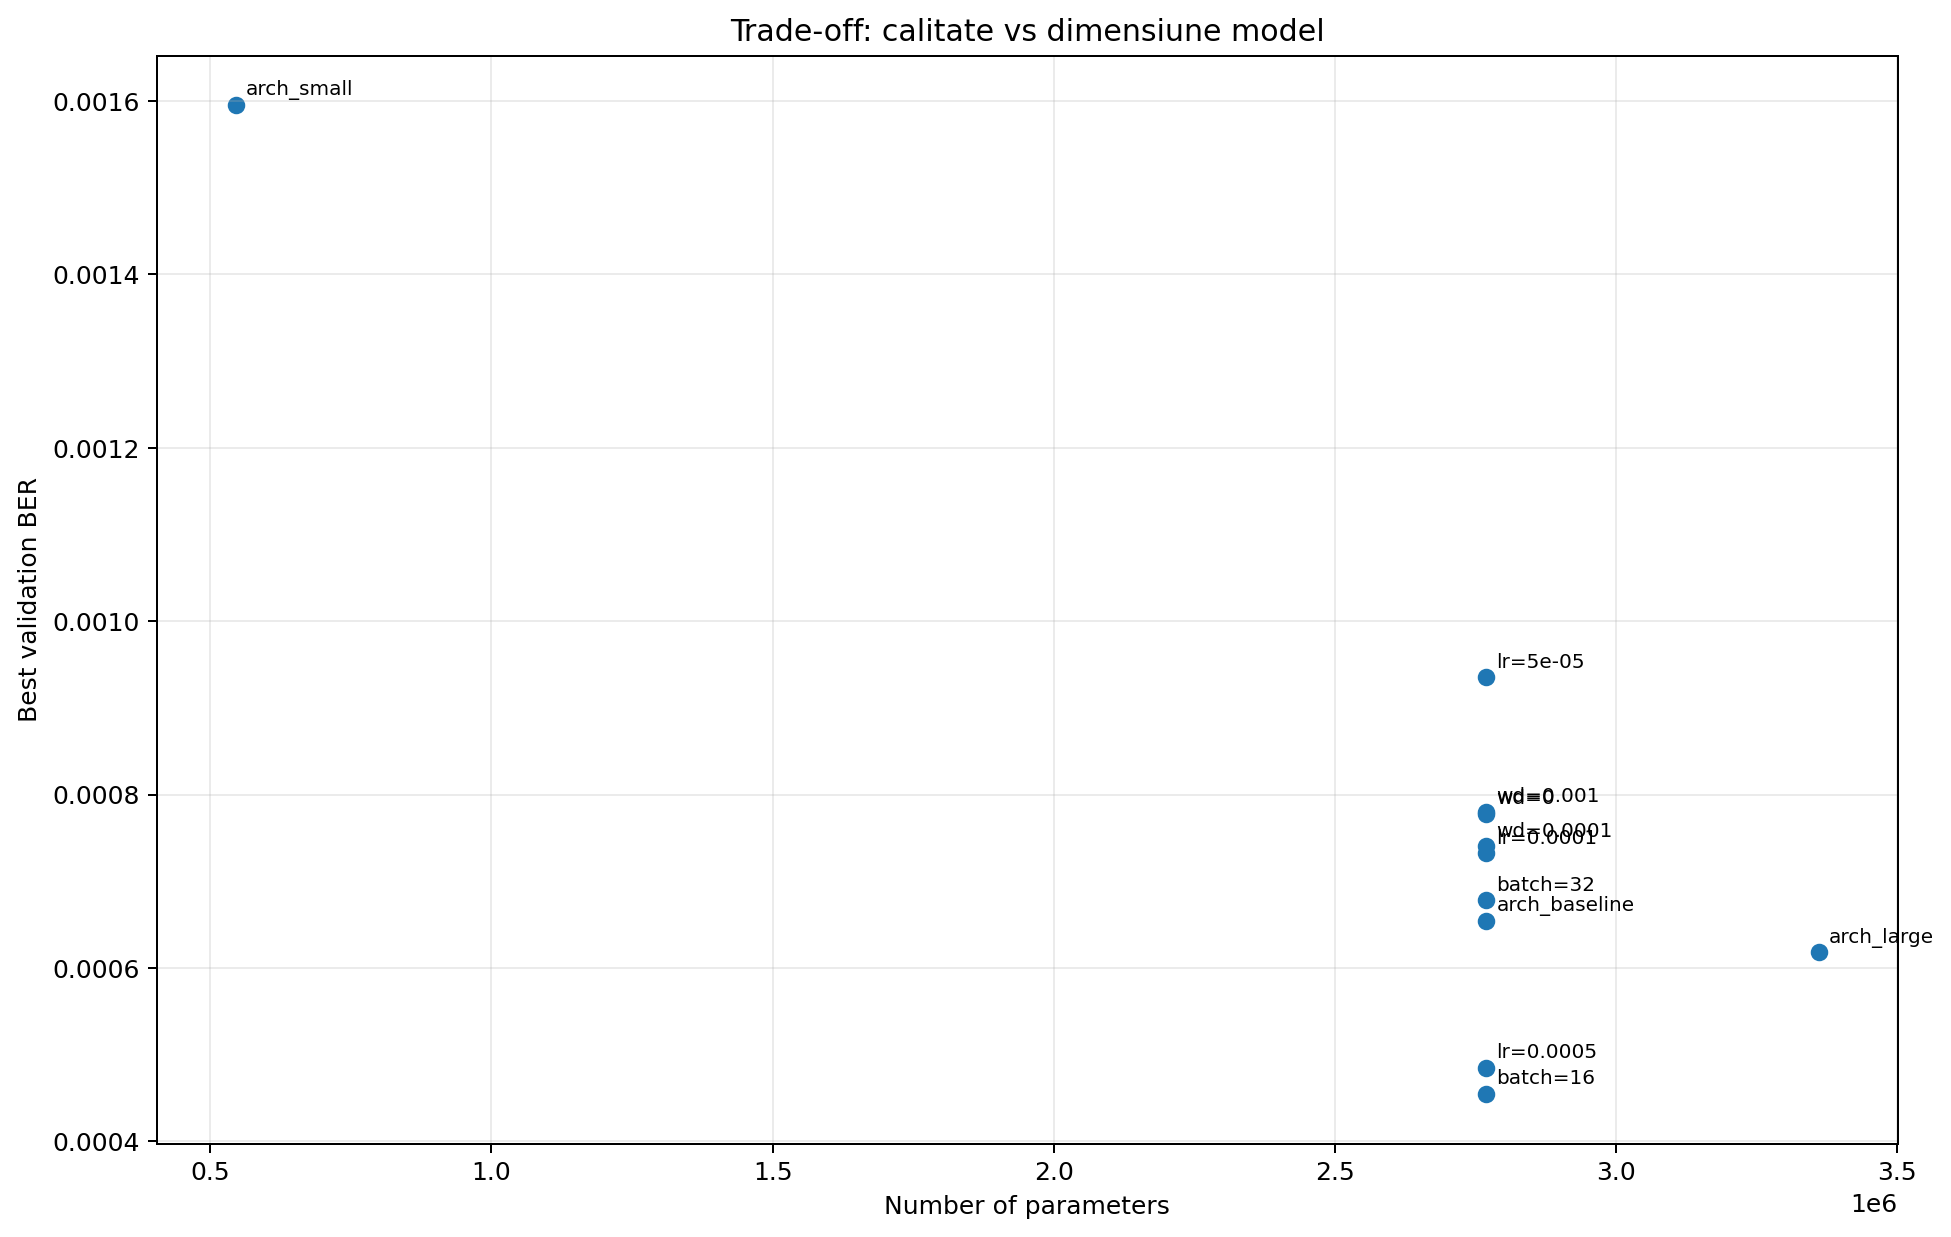
\includegraphics[width=1\textwidth]{images/14_scatter_best_val_ber_vs_parameters.png}
        \caption{Relația dintre BER-ul minim și numărul de parametri}
    \end{minipage}
    \hspace{0.03\textwidth}
    \begin{minipage}{0.48\textwidth}
        \centering
        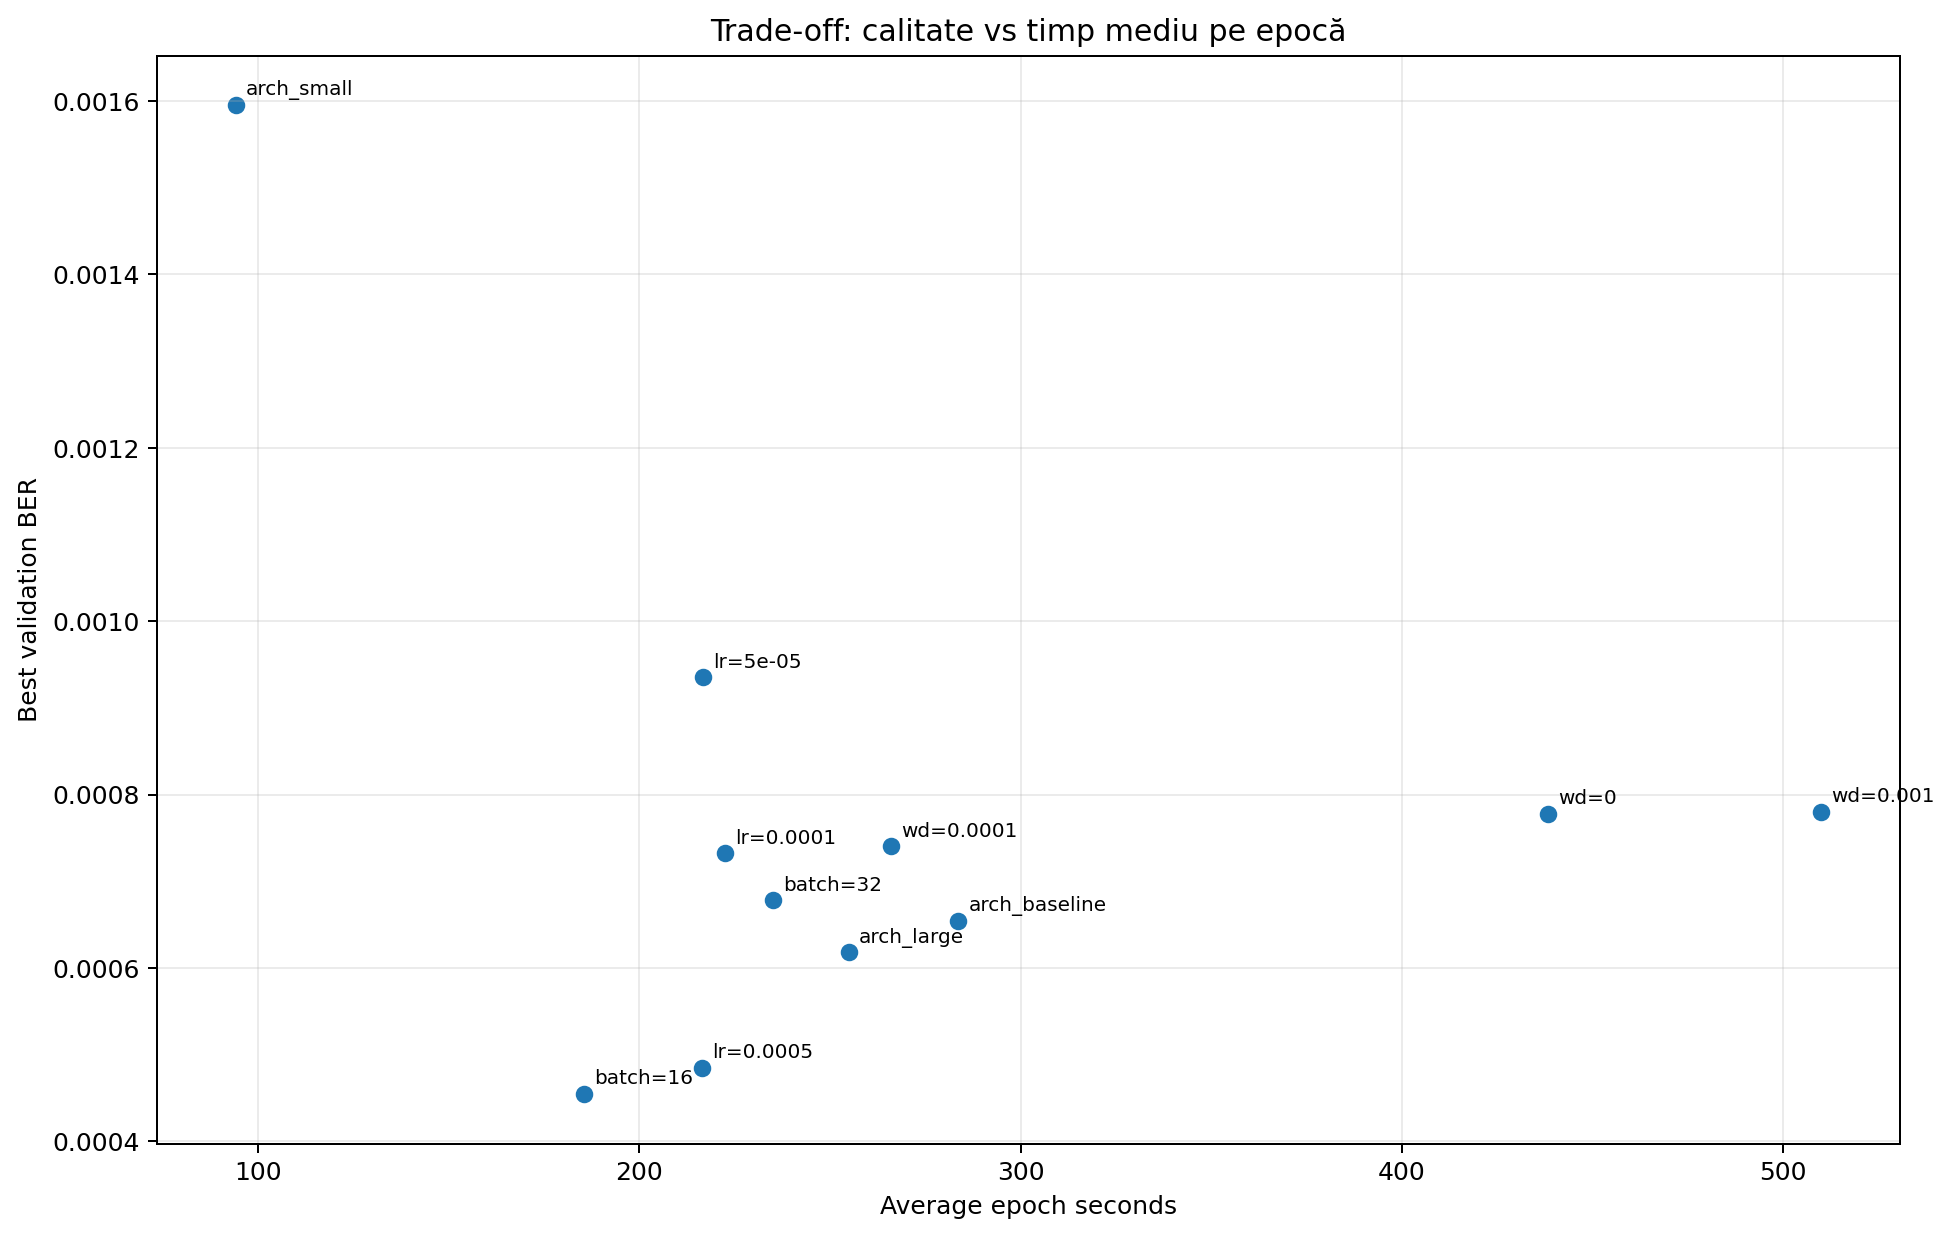
\includegraphics[width=1\textwidth]{images/15_scatter_best_val_ber_vs_avg_epoch_seconds.png}
        \caption{Relația dintre BER-ul minim și timpul mediu pe epocă}
    \end{minipage}
\end{figure}
\FloatBarrier

A fost analizată și stabilitatea antrenării. Pentru fiecare experiment s-a comparat valoarea finală a metricii $val\_ber$ cu cea mai bună valoare obținută în timpul antrenării. O diferență mică între aceste două valori indică faptul că modelul rămâne stabil până la finalul celor $30$ de epoci. Unele configurații au obținut cel mai bun rezultat chiar în ultima epocă, de exemplu $lr = 5 \cdot 10^{-5}$, $weightDecay = 10^{-4}$, $weightDecay = 10^{-3}$ și \textit{arch\_small}. Totuși, acestea nu au fost cele mai bune configurații ca performanță absolută.

Cel mai stabil experiment pe ultimele $5$ epoci a fost configurația fără weight decay, care a avut o deviație standard a $val\_ber$ egală cu $0.00008770$. Aceasta nu a fost însă configurația cu cel mai mic BER, ceea ce arată că stabilitatea finală și performanța maximă nu coincid întotdeauna.

\begin{figure}[htbp]
    \centering
    \begin{minipage}{0.48\textwidth}
        \centering
        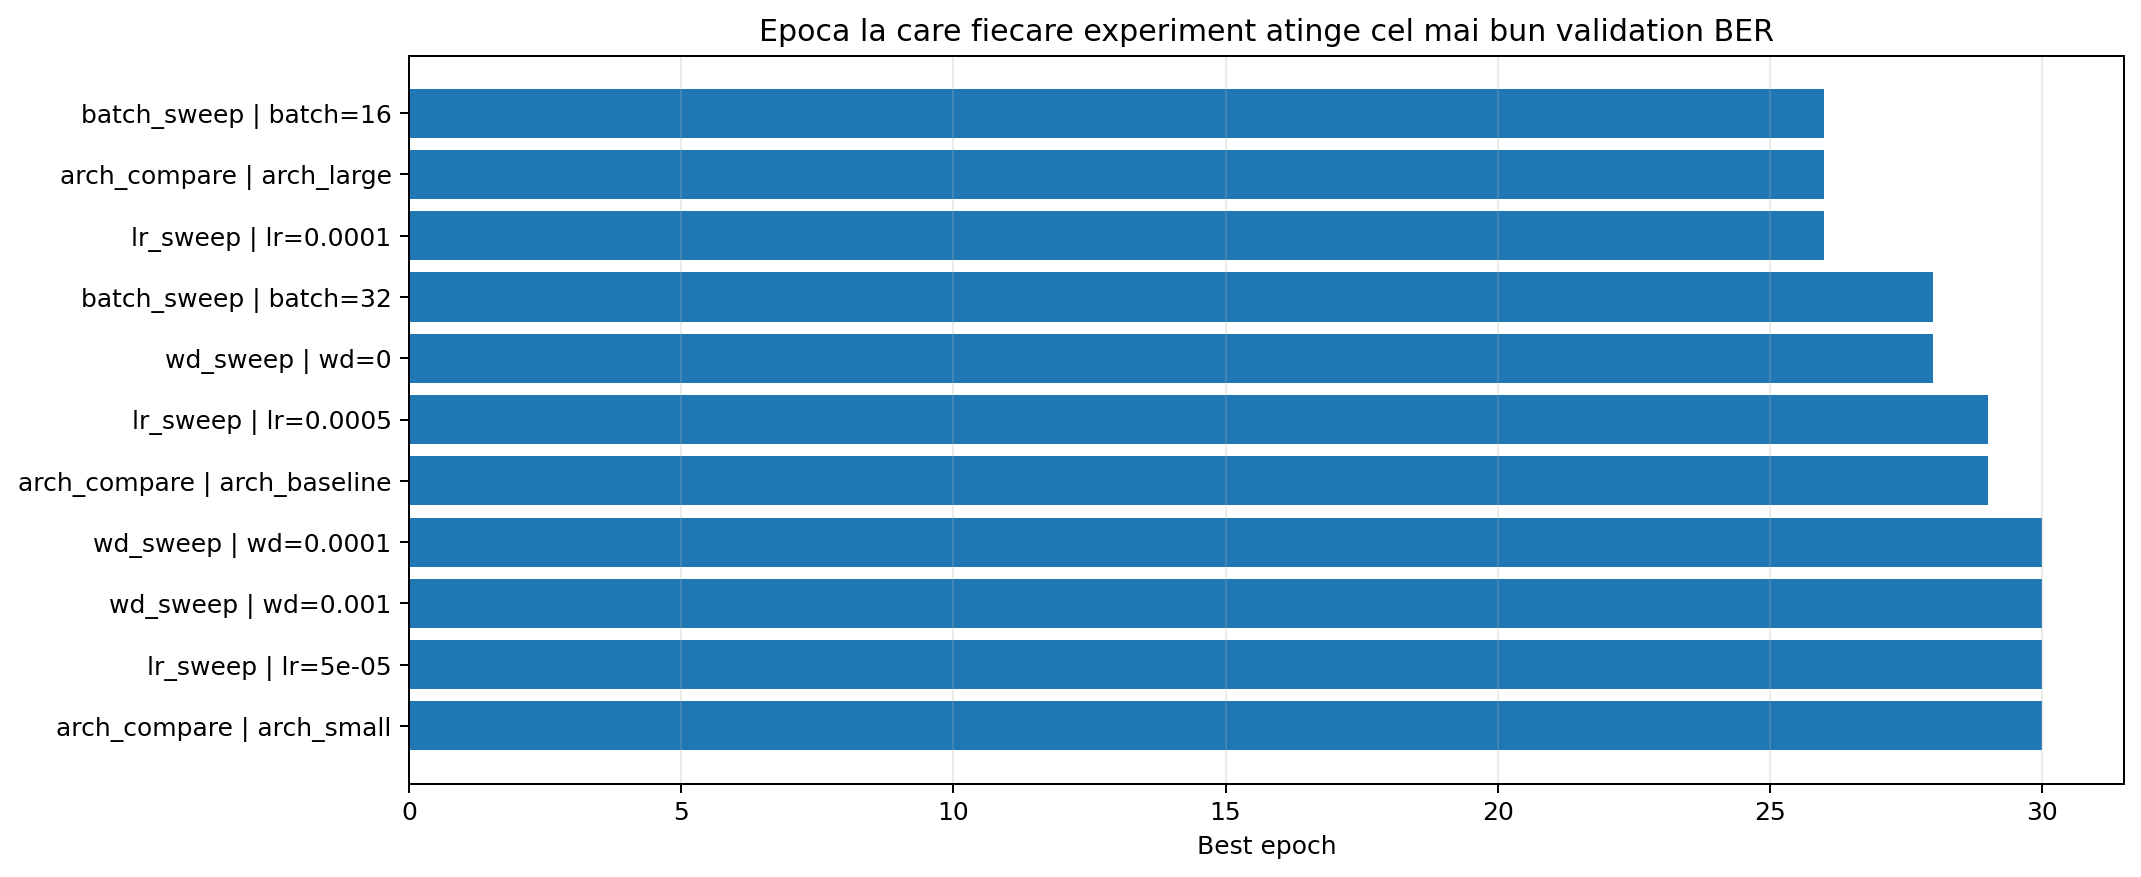
\includegraphics[width=1\textwidth]{images/16_best_epoch_by_experiment.png}
        \caption{Epoca la care fiecare experiment atinge cel mai bun BER}
    \end{minipage}
    \hspace{0.03\textwidth}
    \begin{minipage}{0.48\textwidth}
        \centering
        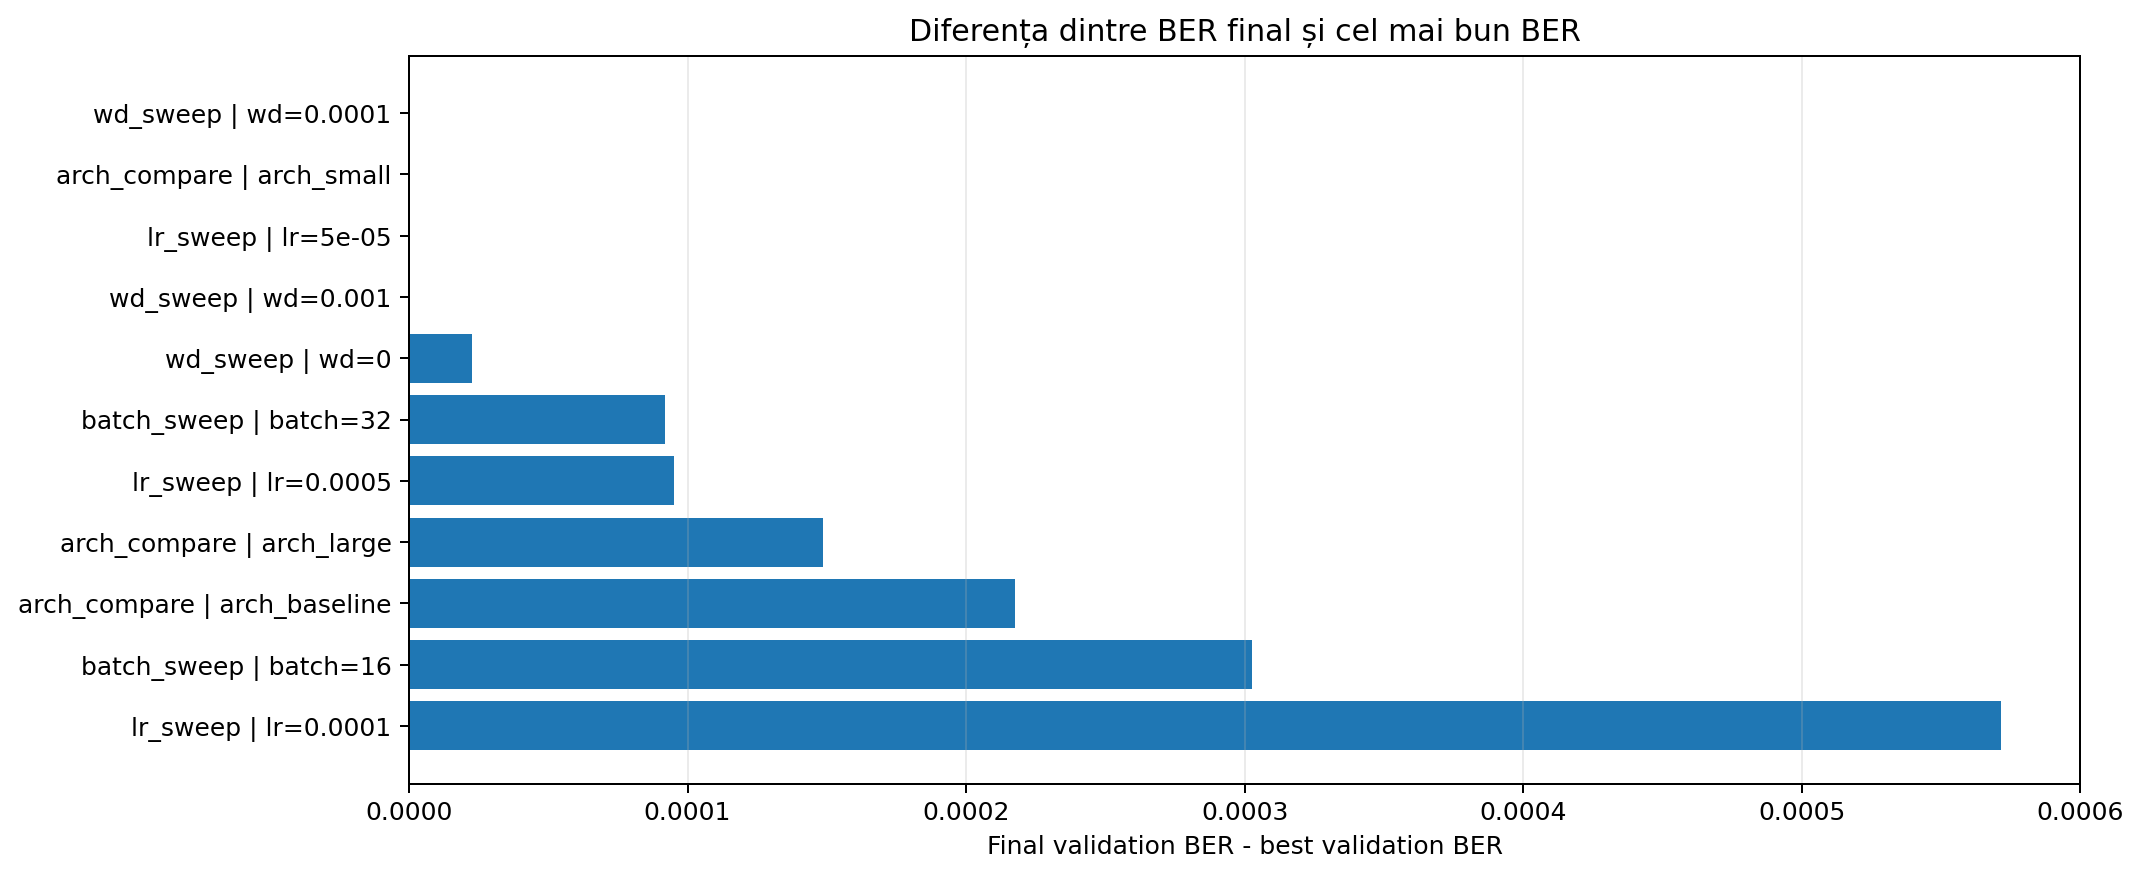
\includegraphics[width=1\textwidth]{images/17_final_minus_best_val_ber.png}
        \caption{Diferența dintre BER-ul final și cel mai bun BER obținut}
    \end{minipage}
\end{figure}
\FloatBarrier

\begin{figure}[htbp]
    \centering
    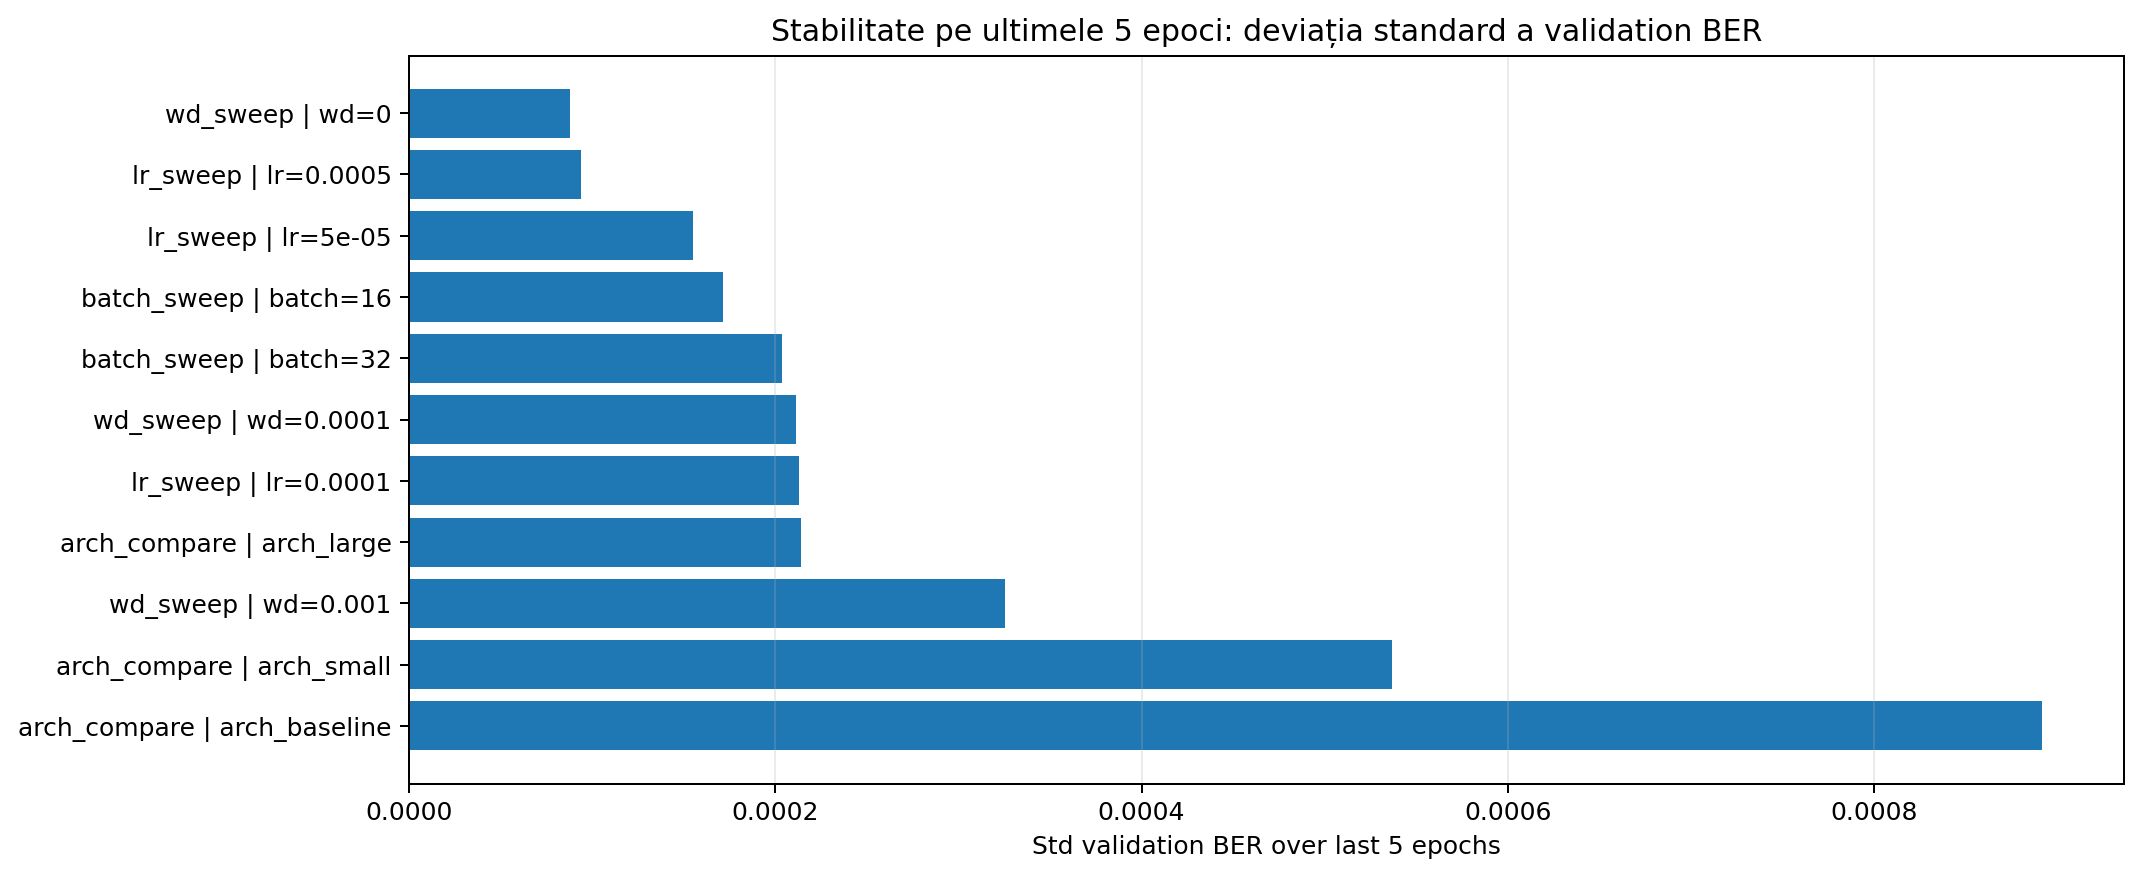
\includegraphics[width=0.7\textwidth]{images/18_last_5_val_ber_std.png}
    \caption{Deviația standard a BER-ului pe ultimele 5 epoci}
\end{figure}
\FloatBarrier

În urma experimentelor, configurația aleasă ca model final este \textit{batch\_sweep\_\_base\_\_batch\_16}, deoarece a obținut cea mai mică rată a erorii la nivel de bit pe setul de validare. Deși configurația cu $lr = 5 \cdot 10^{-4}$ a fost foarte apropiată, diferența de BER favorizează modelul cu batch size $16$.

\[
    Experiment_{final} = batch\_sweep\_\_base\_\_batch\_16
\]

\[
    BER_{final} = 0.00045465
\]

\[
    BitAccuracy_{final} \approx 99.9545\%
\]

\[
    \overline{erori}_{QR} = 0.2005
\]

Aceste rezultate arată că modelul QRBitNet reușește să reconstruiască matricea QR cu o acuratețe foarte ridicată la nivel de modul. Față de rezultatele anterioare, noua configurație experimentală folosește un set de date mai mare, o arhitectură mai complexă și o comparație mai clară între hiperparametri. Cel mai bun model greșește, în medie, aproximativ un bit la fiecare cinci coduri QR din setul de validare, ceea ce indică o capacitate foarte bună de reconstrucție binară.

Totuși, trebuie menționat că aceste rezultate sunt raportate pe setul de validare, nu pe un set de test separat. Prin urmare, ele sunt potrivite pentru compararea configurațiilor și alegerea modelului final, dar performanța finală a sistemului ar trebui confirmată ulterior și pe un set de test independent. Chiar și în aceste condiții, valorile obținute pentru $val\_ber$ și pentru numărul mediu de erori pe cod QR demonstrează că modelul învață structura codurilor QR și poate produce matrici binare foarte apropiate de cele reale.

\section{Concluzii}

Lucrarea de față a avut ca obiectiv dezvoltarea unui sistem inteligent pentru extracția și interpretarea informației vizuale din imagini în condiții de zgomot și incertitudine, obiectiv care a fost atins prin proiectarea și implementarea unei aplicații software complete dedicate managementului automatizat al accesului într-o parcare. Rezultatul obținut confirmă faptul că această problemă poate fi abordată eficient prin combinarea metodelor clasice de procesare a imaginilor cu tehnici moderne de învățare automată și prin integrarea acestora într-o arhitectură software unitară.

Una dintre concluziile principale ale lucrării este că tratarea explicită a zgomotului și a incertitudinii din imaginile de intrare este esențială pentru obținerea unor rezultate robuste în aplicații reale. În scenarii practice, informația vizuală nu este disponibilă într-o formă ideală, iar performanța sistemului depinde de capacitatea acestuia de a corecta, filtra, rectifica și interpreta datele afectate de factori perturbatori. În acest sens, lucrarea arată că procesarea de imagine nu reprezintă doar o etapă auxiliară, ci o componentă fundamentală în pregătirea informației pentru interpretarea automată.

Contribuția centrală a disertației constă în dezvoltarea și integrarea unui pipeline pentru detectarea și decodarea codurilor QR, pipeline care reflectă în mod direct tema lucrării. În cadrul acestuia, informația vizuală este extrasă progresiv din imagini printr-o succesiune de etape: preprocesare, localizare a regiunilor candidate, rectificare geometrică, reconstrucție a structurii codului și decodare finală. Această organizare demonstrează că interpretarea informației vizuale în condiții dificile nu se reduce la o singură operație de recunoaștere, ci presupune un proces compus, în care fiecare etapă contribuie la reducerea incertitudinii și la creșterea calității rezultatului final.

O altă concluzie importantă este că abordarea hibridă adoptată în lucrare este justificată și eficientă. Metodele clasice de procesare a imaginilor oferă control, interpretabilitate și eficiență în localizarea și normalizarea regiunilor de interes, în timp ce modelul bazat pe învățare automată oferă robustețe suplimentară în reconstruirea matricei codului QR atunci când imaginea este afectată de degradări semnificative. Prin urmare, lucrarea susține ideea că, în probleme de extracție și interpretare a informației vizuale din imagini incerte, cele mai bune rezultate pot fi obținute prin complementaritatea dintre metodele deterministe și cele bazate pe date.

Rezultatele obținute evidențiază și importanța integrării practice a componentelor dezvoltate. Modelul de învățare automată nu rămâne la nivel de experiment, ci este inclus efectiv în aplicația finală prin export în format ONNX și utilizare în mediul C++. Această tranziție de la faza de cercetare și antrenare la integrarea într-un sistem software operațional reprezintă o contribuție importantă a lucrării și confirmă fezabilitatea utilizării unor modele proprii în aplicații inginerești reale.

Dincolo de componenta de analiză vizuală, lucrarea confirmă utilitatea unei arhitecturi software distribuite. Backend-ul responsabil de comunicațiile HTTP și WebSocket, mecanismele de securizare, baza de date pentru persistența informațiilor, aplicația desktop și aplicația web contribuie împreună la transformarea unei soluții algoritmice într-un sistem complet, capabil să răspundă unor cerințe funcționale reale. Această integrare arată că interpretarea informației vizuale devine cu adevărat valoroasă atunci când rezultatele pot fi utilizate imediat în procese operaționale, de monitorizare și de administrare.

Totodată, lucrarea evidențiază evoluția unui proiect anterior către o soluție mai matură și mai generală. Dacă etapa precedentă era axată în principal pe recunoașterea numerelor de înmatriculare, actuala disertație deplasează accentul către interpretarea robustă a codurilor QR, ceea ce extinde domeniul aplicației și consolidează caracterul său de sistem inteligent de analiză vizuală. Această evoluție reflectă o trecere de la o problemă specifică de recunoaștere textuală la o problemă mai largă de reconstrucție și interpretare a informației vizuale în condiții dificile.

În concluzie, lucrarea demonstrează că dezvoltarea unui sistem inteligent pentru extracția și interpretarea informației vizuale din imagini în condiții de zgomot și incertitudine este nu doar posibilă, ci și practică în contextul unei aplicații reale. Soluția propusă oferă un exemplu concret de integrare a procesării imaginilor, a învățării automate și a ingineriei software într-un produs coerent, robust și extensibil. Componenta de detecție și decodare a codurilor QR constituie contribuția originală principală, iar rezultatele obținute confirmă relevanța unei astfel de abordări pentru dezvoltarea viitoare a sistemelor inteligente bazate pe analiză vizuală.

Ca direcții viitoare, sistemul poate fi extins prin diversificarea seturilor de date utilizate la antrenare, îmbunătățirea rezistenței la degradări mai severe, generalizarea către alte tipuri de coduri bidimensionale și integrarea unor mecanisme suplimentare de decizie automată. Prin aceste extinderi, aplicația poate evolua către o platformă și mai performantă pentru interpretarea automată a informației vizuale în medii reale, caracterizate prin variabilitate, zgomot și incertitudine.
